% Options for packages loaded elsewhere
\PassOptionsToPackage{unicode}{hyperref}
\PassOptionsToPackage{hyphens}{url}
\documentclass[
  ignorenonframetext,
]{beamer}
\newif\ifbibliography
\usepackage{pgfpages}
\setbeamertemplate{caption}[numbered]
\setbeamertemplate{caption label separator}{: }
\setbeamercolor{caption name}{fg=normal text.fg}
\beamertemplatenavigationsymbolsempty
% remove section numbering
\setbeamertemplate{part page}{
  \centering
  \begin{beamercolorbox}[sep=16pt,center]{part title}
    \usebeamerfont{part title}\insertpart\par
  \end{beamercolorbox}
}
\setbeamertemplate{section page}{
  \centering
  \begin{beamercolorbox}[sep=12pt,center]{section title}
    \usebeamerfont{section title}\insertsection\par
  \end{beamercolorbox}
}
\setbeamertemplate{subsection page}{
  \centering
  \begin{beamercolorbox}[sep=8pt,center]{subsection title}
    \usebeamerfont{subsection title}\insertsubsection\par
  \end{beamercolorbox}
}
% Prevent slide breaks in the middle of a paragraph
\widowpenalties 1 10000
\raggedbottom
\AtBeginPart{
  \frame{\partpage}
}
\AtBeginSection{
  \ifbibliography
  \else
    \frame{\sectionpage}
  \fi
}
\AtBeginSubsection{
  \frame{\subsectionpage}
}
\usepackage{iftex}
\ifPDFTeX
  \usepackage[T1]{fontenc}
  \usepackage[utf8]{inputenc}
  \usepackage{textcomp} % provide euro and other symbols
\else % if luatex or xetex
  \usepackage{unicode-math} % this also loads fontspec
  \defaultfontfeatures{Scale=MatchLowercase}
  \defaultfontfeatures[\rmfamily]{Ligatures=TeX,Scale=1}
\fi
\usepackage{lmodern}
\ifPDFTeX\else
  % xetex/luatex font selection
\fi
% Use upquote if available, for straight quotes in verbatim environments
\IfFileExists{upquote.sty}{\usepackage{upquote}}{}
\IfFileExists{microtype.sty}{% use microtype if available
  \usepackage[]{microtype}
  \UseMicrotypeSet[protrusion]{basicmath} % disable protrusion for tt fonts
}{}
\makeatletter
\@ifundefined{KOMAClassName}{% if non-KOMA class
  \IfFileExists{parskip.sty}{%
    \usepackage{parskip}
  }{% else
    \setlength{\parindent}{0pt}
    \setlength{\parskip}{6pt plus 2pt minus 1pt}}
}{% if KOMA class
  \KOMAoptions{parskip=half}}
\makeatother
\usepackage{longtable,booktabs,array}
\newcounter{none} % for unnumbered tables
\usepackage{calc} % for calculating minipage widths
\usepackage{caption}
% Make caption package work with longtable
\makeatletter
\def\fnum@table{\tablename~\thetable}
\makeatother
\usepackage{graphicx}
\makeatletter
\newsavebox\pandoc@box
\newcommand*\pandocbounded[1]{% scales image to fit in text height/width
  \sbox\pandoc@box{#1}%
  \Gscale@div\@tempa{\textheight}{\dimexpr\ht\pandoc@box+\dp\pandoc@box\relax}%
  \Gscale@div\@tempb{\linewidth}{\wd\pandoc@box}%
  \ifdim\@tempb\p@<\@tempa\p@\let\@tempa\@tempb\fi% select the smaller of both
  \ifdim\@tempa\p@<\p@\scalebox{\@tempa}{\usebox\pandoc@box}%
  \else\usebox{\pandoc@box}%
  \fi%
}
% Set default figure placement to htbp
\def\fps@figure{htbp}
\makeatother
\setlength{\emergencystretch}{3em} % prevent overfull lines
\providecommand{\tightlist}{%
  \setlength{\itemsep}{0pt}\setlength{\parskip}{0pt}}
% Auto-generated by infrastructure/rendering/_pdf_latex_helpers.py::extract_math_font_preamble.
% Minimal header passed to Pandoc via -H so Beamer slides pick up the same math font
% as the combined-PDF path. Adjust the manuscript's preamble.md to change the font globally.
\usepackage{unicode-math}
\setmathfont{latinmodern-math.otf}

% Slide layout defaults for warning-clean scientific decks.
\usepackage{etoolbox}
\IfFileExists{xurl.sty}{\usepackage{xurl}}{}
\IfFileExists{seqsplit.sty}{\usepackage{seqsplit}}{\newcommand{\seqsplit}[1]{#1}}
\protected\def\breakseq#1{\seqsplit{#1}}
\protected\def\breaktt#1{\begingroup\ttfamily\seqsplit{#1}\endgroup}
\setlength{\emergencystretch}{6em}
\tolerance=5000
\hbadness=10000
\hfuzz=1pt
\setlength{\tabcolsep}{2pt}
\AtBeginEnvironment{longtable}{\tiny\renewcommand{\arraystretch}{0.86}\setlength{\tabcolsep}{1pt}}
\AtBeginEnvironment{tabular}{\tiny\renewcommand{\arraystretch}{0.86}\setlength{\tabcolsep}{1pt}}

% Natbib and cross-reference fallbacks — slides don't load natbib
% or cleveref, but combined-PDF manuscript prose may emit these
% commands. The fallback renders citations as a bracketed key list
% and cross-references as detokenized labels so slides don't fail on
% undefined control sequences or raw underscores. \providecommand is
% a no-op if packages load later.
\providecommand{\citep}[1]{[#1]}
\providecommand{\citet}[1]{#1}
\providecommand{\citealp}[1]{#1}
\providecommand{\citeauthor}[1]{#1}
\providecommand{\citeyear}[1]{#1}
\providecommand{\cref}[1]{\texttt{\detokenize{#1}}}
\providecommand{\Cref}[1]{\texttt{\detokenize{#1}}}

\newtheorem{proposition}{Proposition}
\newtheorem{hypothesis}{Hypothesis}
\usepackage{bookmark}
\IfFileExists{xurl.sty}{\usepackage{xurl}}{} % add URL line breaks if available
\urlstyle{same}
% fallback for those not using the hyperref driver hyperxmp:
\makeatletter
\@ifundefined{xmpquote}{\newcommand{\xmpquote}[1]{#1}}{}
\makeatother
\hypersetup{
  hidelinks,
  pdfcreator={LaTeX via pandoc}}

\author{\texorpdfstring{}{}}
\date{}

\begin{document}

\section{Publication Atlas, Caption Contract, and Scholarship
Audit}\label{sec:publication_audit}

\begin{frame}[allowframebreaks]{Publication Atlas, Caption Contract, and
Scholarship Audit}
The publication layer is generated from the same typed package state as
the stimuli. It contains 15 scientific figures, 10 machine-readable
tables, and a separately provenance-recorded editorial cover. The cover
is an illustration of the project's subject and methods aesthetic; it is
not a stimulus, a participant result, or evidence of a perceptual
effect.
\end{frame}

\begin{frame}[allowframebreaks]{Claim-level visualization}
\protect\phantomsection\label{claim-level-visualization}
\begin{figure}
\centering
\pandocbounded{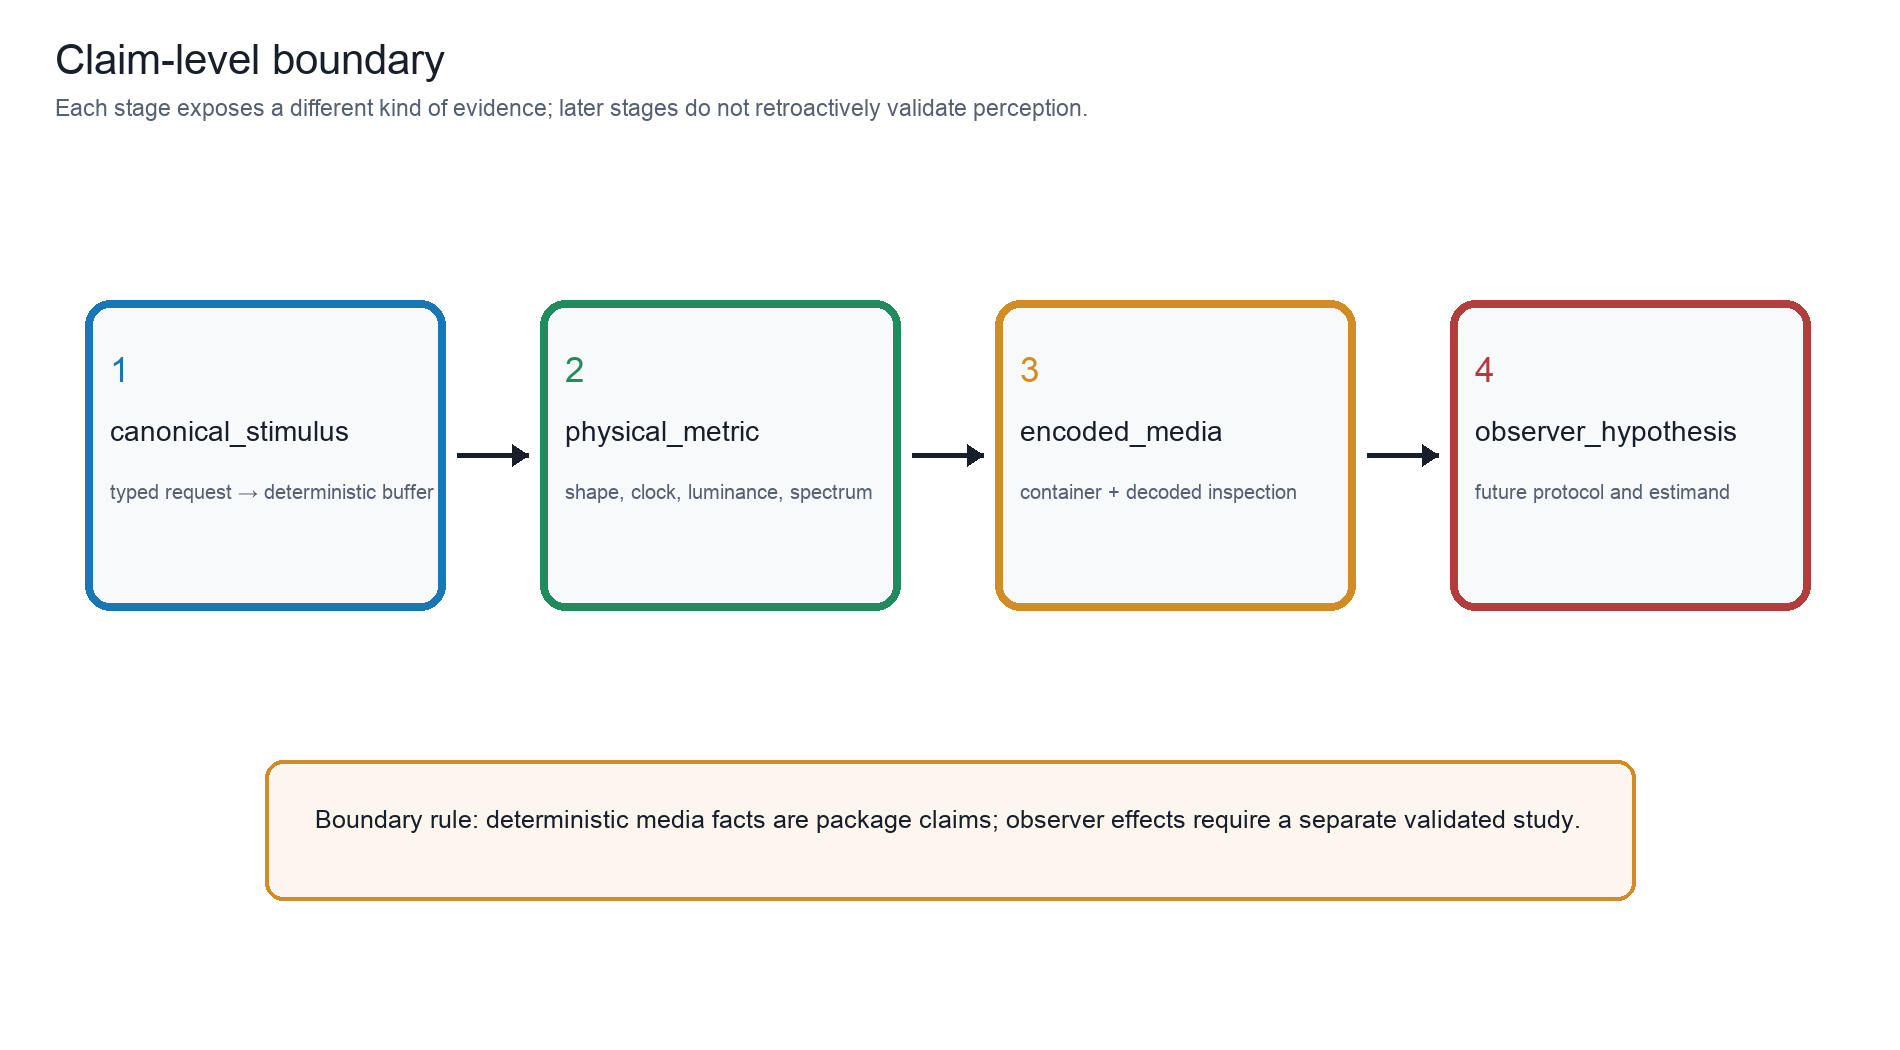
\includegraphics[keepaspectratio,alt={Four numbered boxes separate canonical stimulus, physical metric, encoded media, and observer hypothesis, with a boundary rule stating that observer effects require a separate study.}]{../figures/claim_boundary.png}}
\caption{Four numbered boxes separate canonical stimulus, physical
metric, encoded media, and observer hypothesis, with a boundary rule
stating that observer effects require a separate
study.}\label{fig:claim_boundary}
\end{figure}

What this figure shows: Four numbered boxes separate canonical stimulus,
physical metric, encoded media, and observer hypothesis, with a boundary
rule stating that observer effects require a separate study. The
four-stage boundary distinguishes what DuckRabbit can establish
directly---canonical stimulus identity, physical/media metrics, and
decoded encoded-media facts---from a future observer hypothesis. Source
data output/data/claim\_boundary.json records the stage definitions and
boundary rule; the arrows describe increasing evidential requirements,
not an inference that one stage establishes the next. Controls: claim
levels in the taxonomy and manifest; seed not applicable to the
explanatory diagram. Objective facts: no unit-bearing objective quantity
is applicable; stage definitions and evidence boundaries are preserved
in the sidecar. Claim level: source\_supported. Source data:
output/data/claim\_boundary.json (SHA-256 digest recorded in the figure
registry). Evidence lineage: formalism:eq:observer\_estimand,
formalism:eq:canonical\_digest. Limitations: The diagram is a
documentation contract and does not replace a preregistered observer
study or empirical data. Boundary: A deterministic artifact can support
a future hypothesis but cannot supply the observer data required to test
it.

The claim boundary in \breakseq{[@fig:claim\_boundary]} is a typed epistemic
interface. A canonical digest identifies a deterministic buffer;
objective metrics identify properties of that buffer; encoded-media
verification identifies facts of the delivered file. A future observer
hypothesis is a different object with its own protocol, estimand, and
uncertainty interval.
\end{frame}

\begin{frame}[fragile,allowframebreaks]{Scholarship map and lineage}
\protect\phantomsection\label{scholarship-map-and-lineage}
\begin{figure}
\centering
\pandocbounded{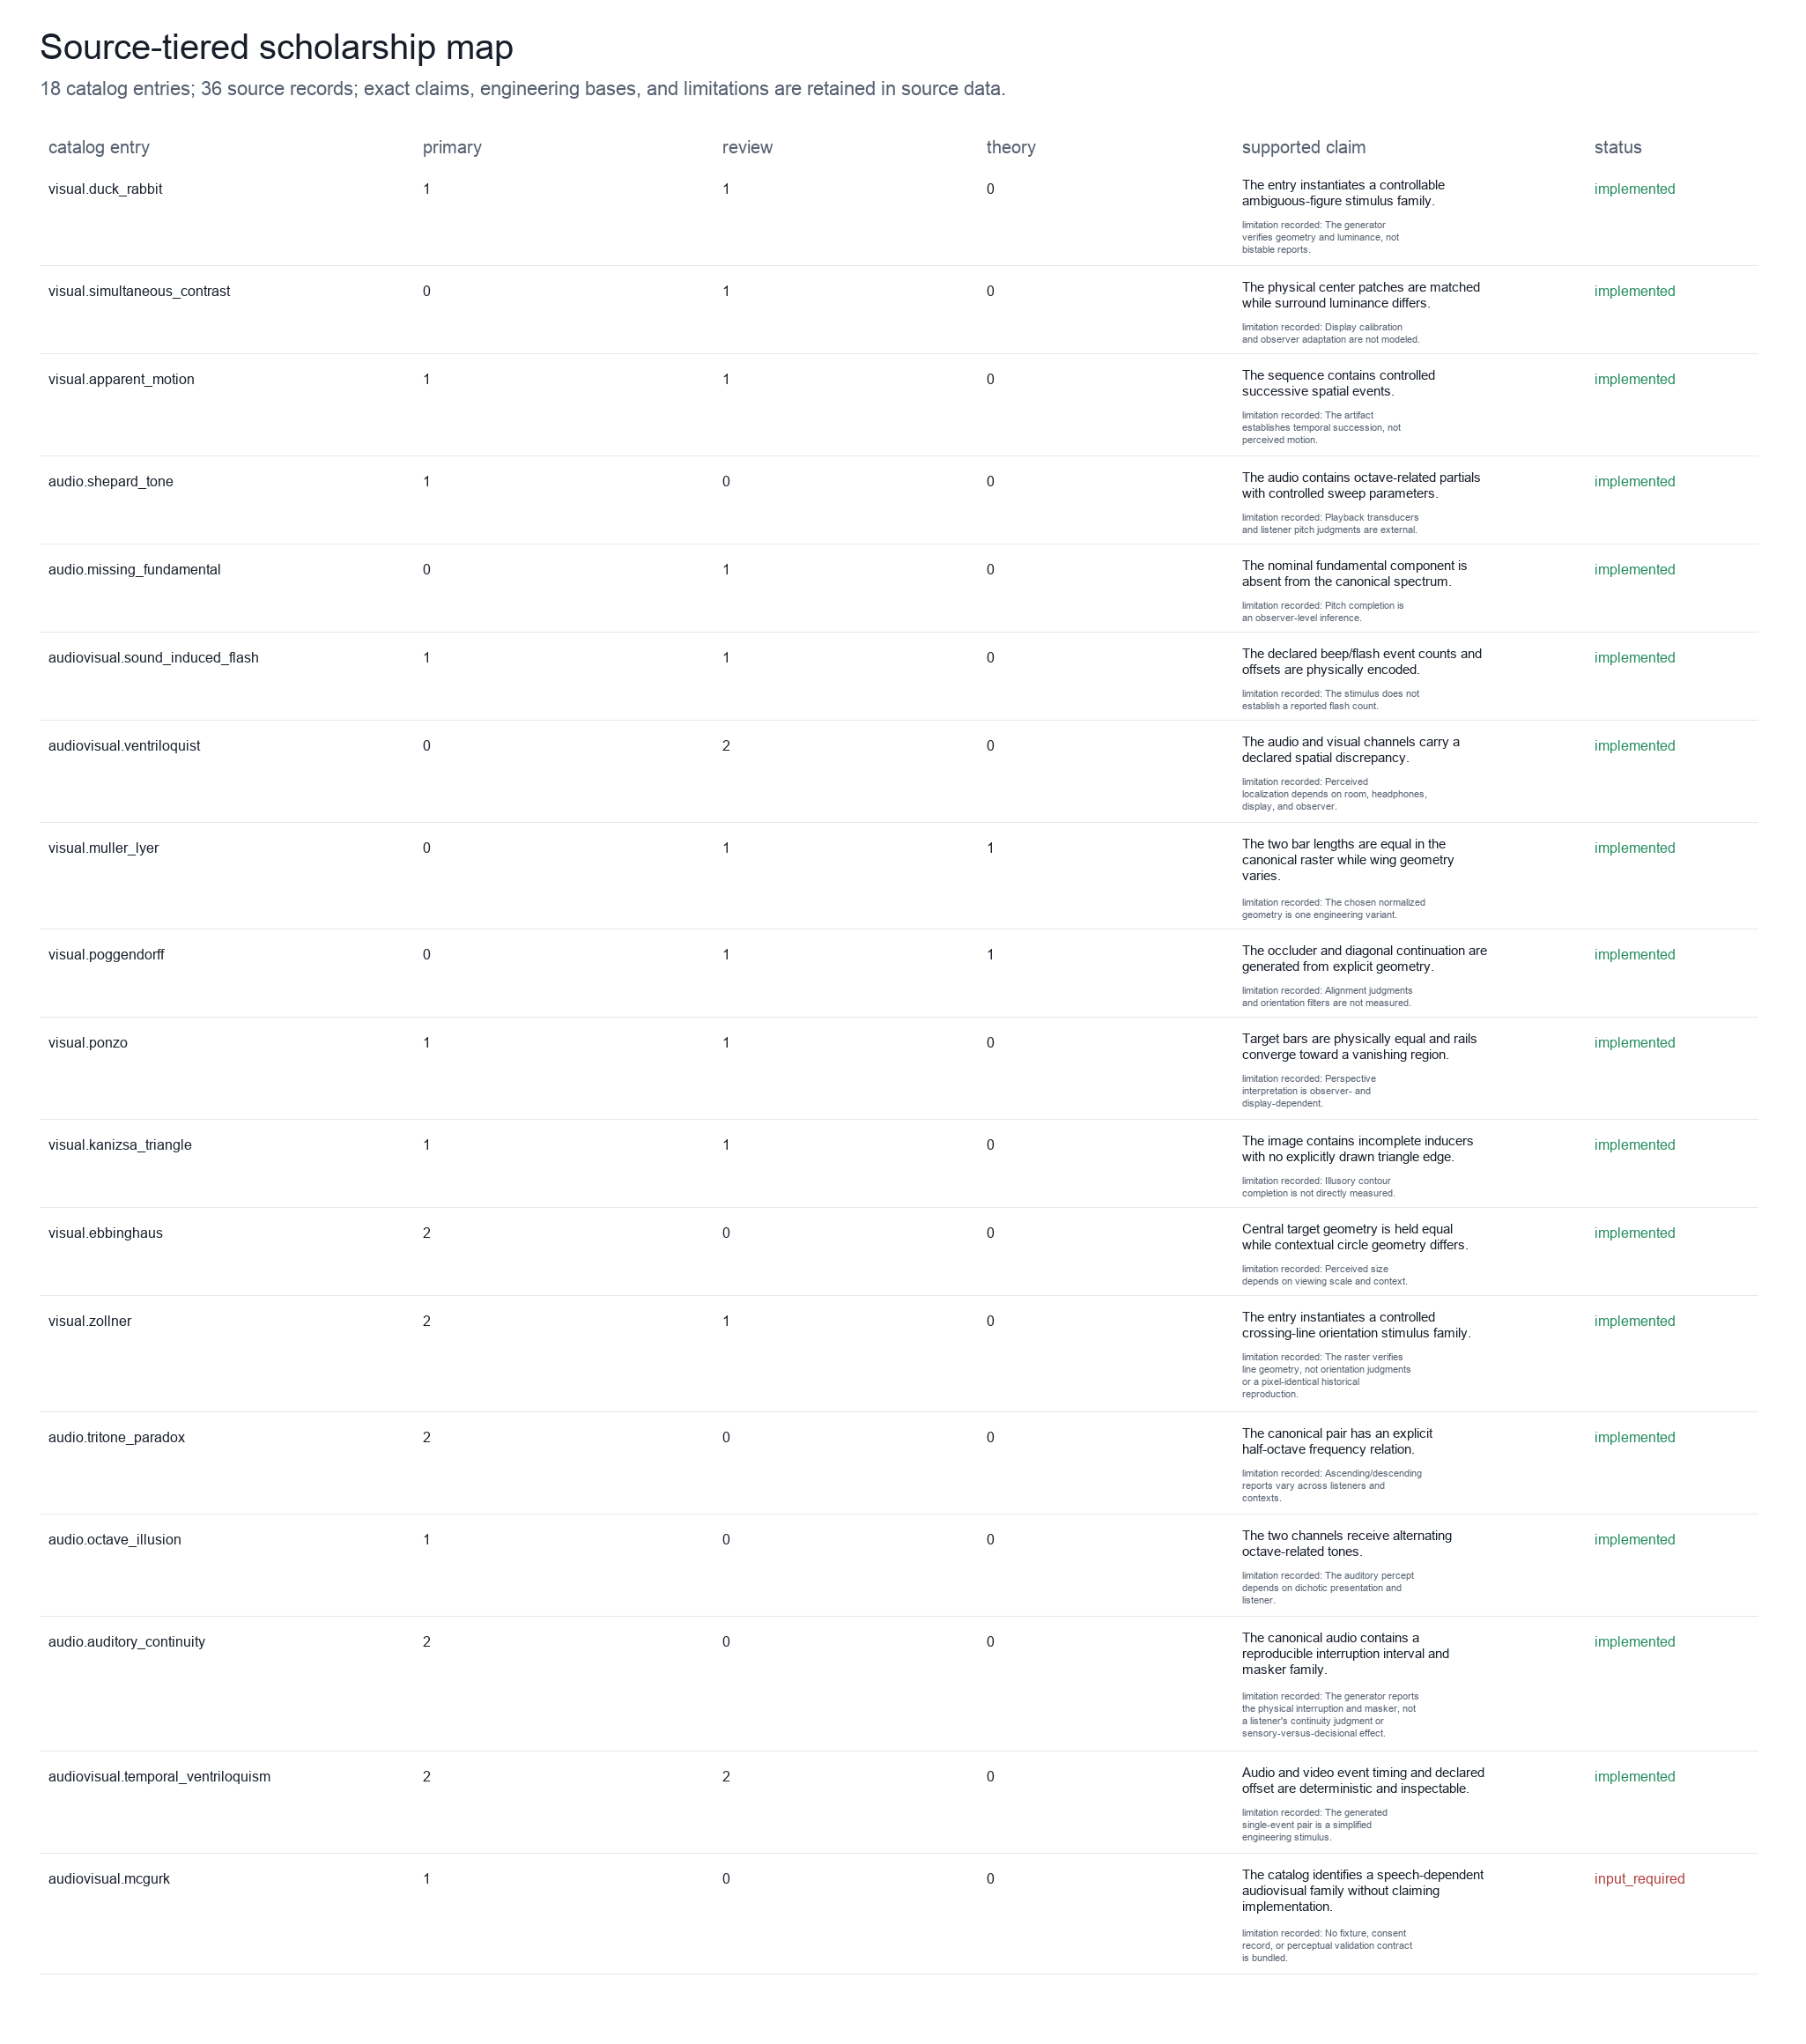
\includegraphics[keepaspectratio,alt={Rows map catalog entries to source tiers, exact supported claims, engineering bases, limitations, and implementation status.}]{../figures/scholarship_map.png}}
\caption{Rows map catalog entries to source tiers, exact supported
claims, engineering bases, limitations, and implementation
status.}\label{fig:scholarship_map}
\end{figure}

What this figure shows: Rows map catalog entries to source tiers, exact
supported claims, engineering bases, limitations, and implementation
status. The map links every catalog entry to its primary, review, and
theory records, then preserves the exact source-supported claim,
engineering departure, limitation, and implementation status. Source
data output/data/scholarship\_map.json are generated from the checked-in
evidence matrix; a source record supports only the statement written in
that record and does not certify pixel- or task-identical replication.
Controls: checked-in evidence matrix; source roles and entry statuses;
audit date recorded in data/evidence\_matrix.json. Objective facts: one
evidence row per catalog entry (18 entries); source-tier counts, exact
claim text, engineering basis, limitation, and gap status. Claim level:
source\_supported. Source data: output/data/scholarship\_map.json
(SHA-256 digest recorded in the figure registry). Evidence lineage:
gregory1997visual, brugger1999duckrabbit, yildiz2022ponzo,
hirst2020sound, bruns2019ventriloquist. Limitations: The offline
snapshot validates citation and lineage structure; live resolver status
is a separate audit, and classifications can remain contested. Boundary:
Scholarship coverage bounds the package's evidence record and does not
establish that any generated stimulus produces a universal percept.

The source map \breakseq{[@fig:scholarship\_map]} and
\breakseq{[@tbl:evidence\_audit]} make five distinctions explicit: a primary
demonstration, a review, a theoretical account, DuckRabbit's engineering
basis, and an evidence limitation. Brugger's duck/rabbit study documents
variation across figure variants and observers; this supports a careful
ambiguity-family record, not a universal bistability claim
\breakseq{[@brugger1999duckrabbit]}. Yildiz et al.~review competing
explanations of Ponzo-like illusions, so the catalog retains both a
geometric construction and an unresolved theoretical boundary
\breakseq{[@yildiz2022ponzo]}. Repp's tritone analysis likewise motivates
listener- and context-sensitive limitations \breakseq{[@repp1997tritone]}.

The audit also treats software and its metadata as part of the scholarly
record. FAIR guidance emphasizes machine-actionable provenance and
reuse, and software-citation principles emphasize crediting an
identifiable version rather than citing an undifferentiated project name
\breakseq{[@wilkinson2016fair; @smith2016software]}. Accordingly, the release
includes \texttt{CITATION.cff}, CodeMeta, Zenodo metadata, versioned
manifests, source-data sidecars, and resolver-linked bibliography
entries. These improve discoverability and attribution; they do not
increase the evidential level of any perceptual claim.

The intended public software identity is explicit: DuckRabbit will be
released at the
\href{https://github.com/docxology/DuckRabbit}{DuckRabbit public GitHub
repository} under the authorship of Daniel Ari Friedman, Active
Inference Institute. The repository URL identifies the future citable
software object; it is not a claim that the private sidecar has already
been publicly mirrored.
\end{frame}

\begin{frame}[allowframebreaks]{Formal traceability and objective
metrics}
\protect\phantomsection\label{formal-traceability-and-objective-metrics}
\begin{figure}
\centering
\pandocbounded{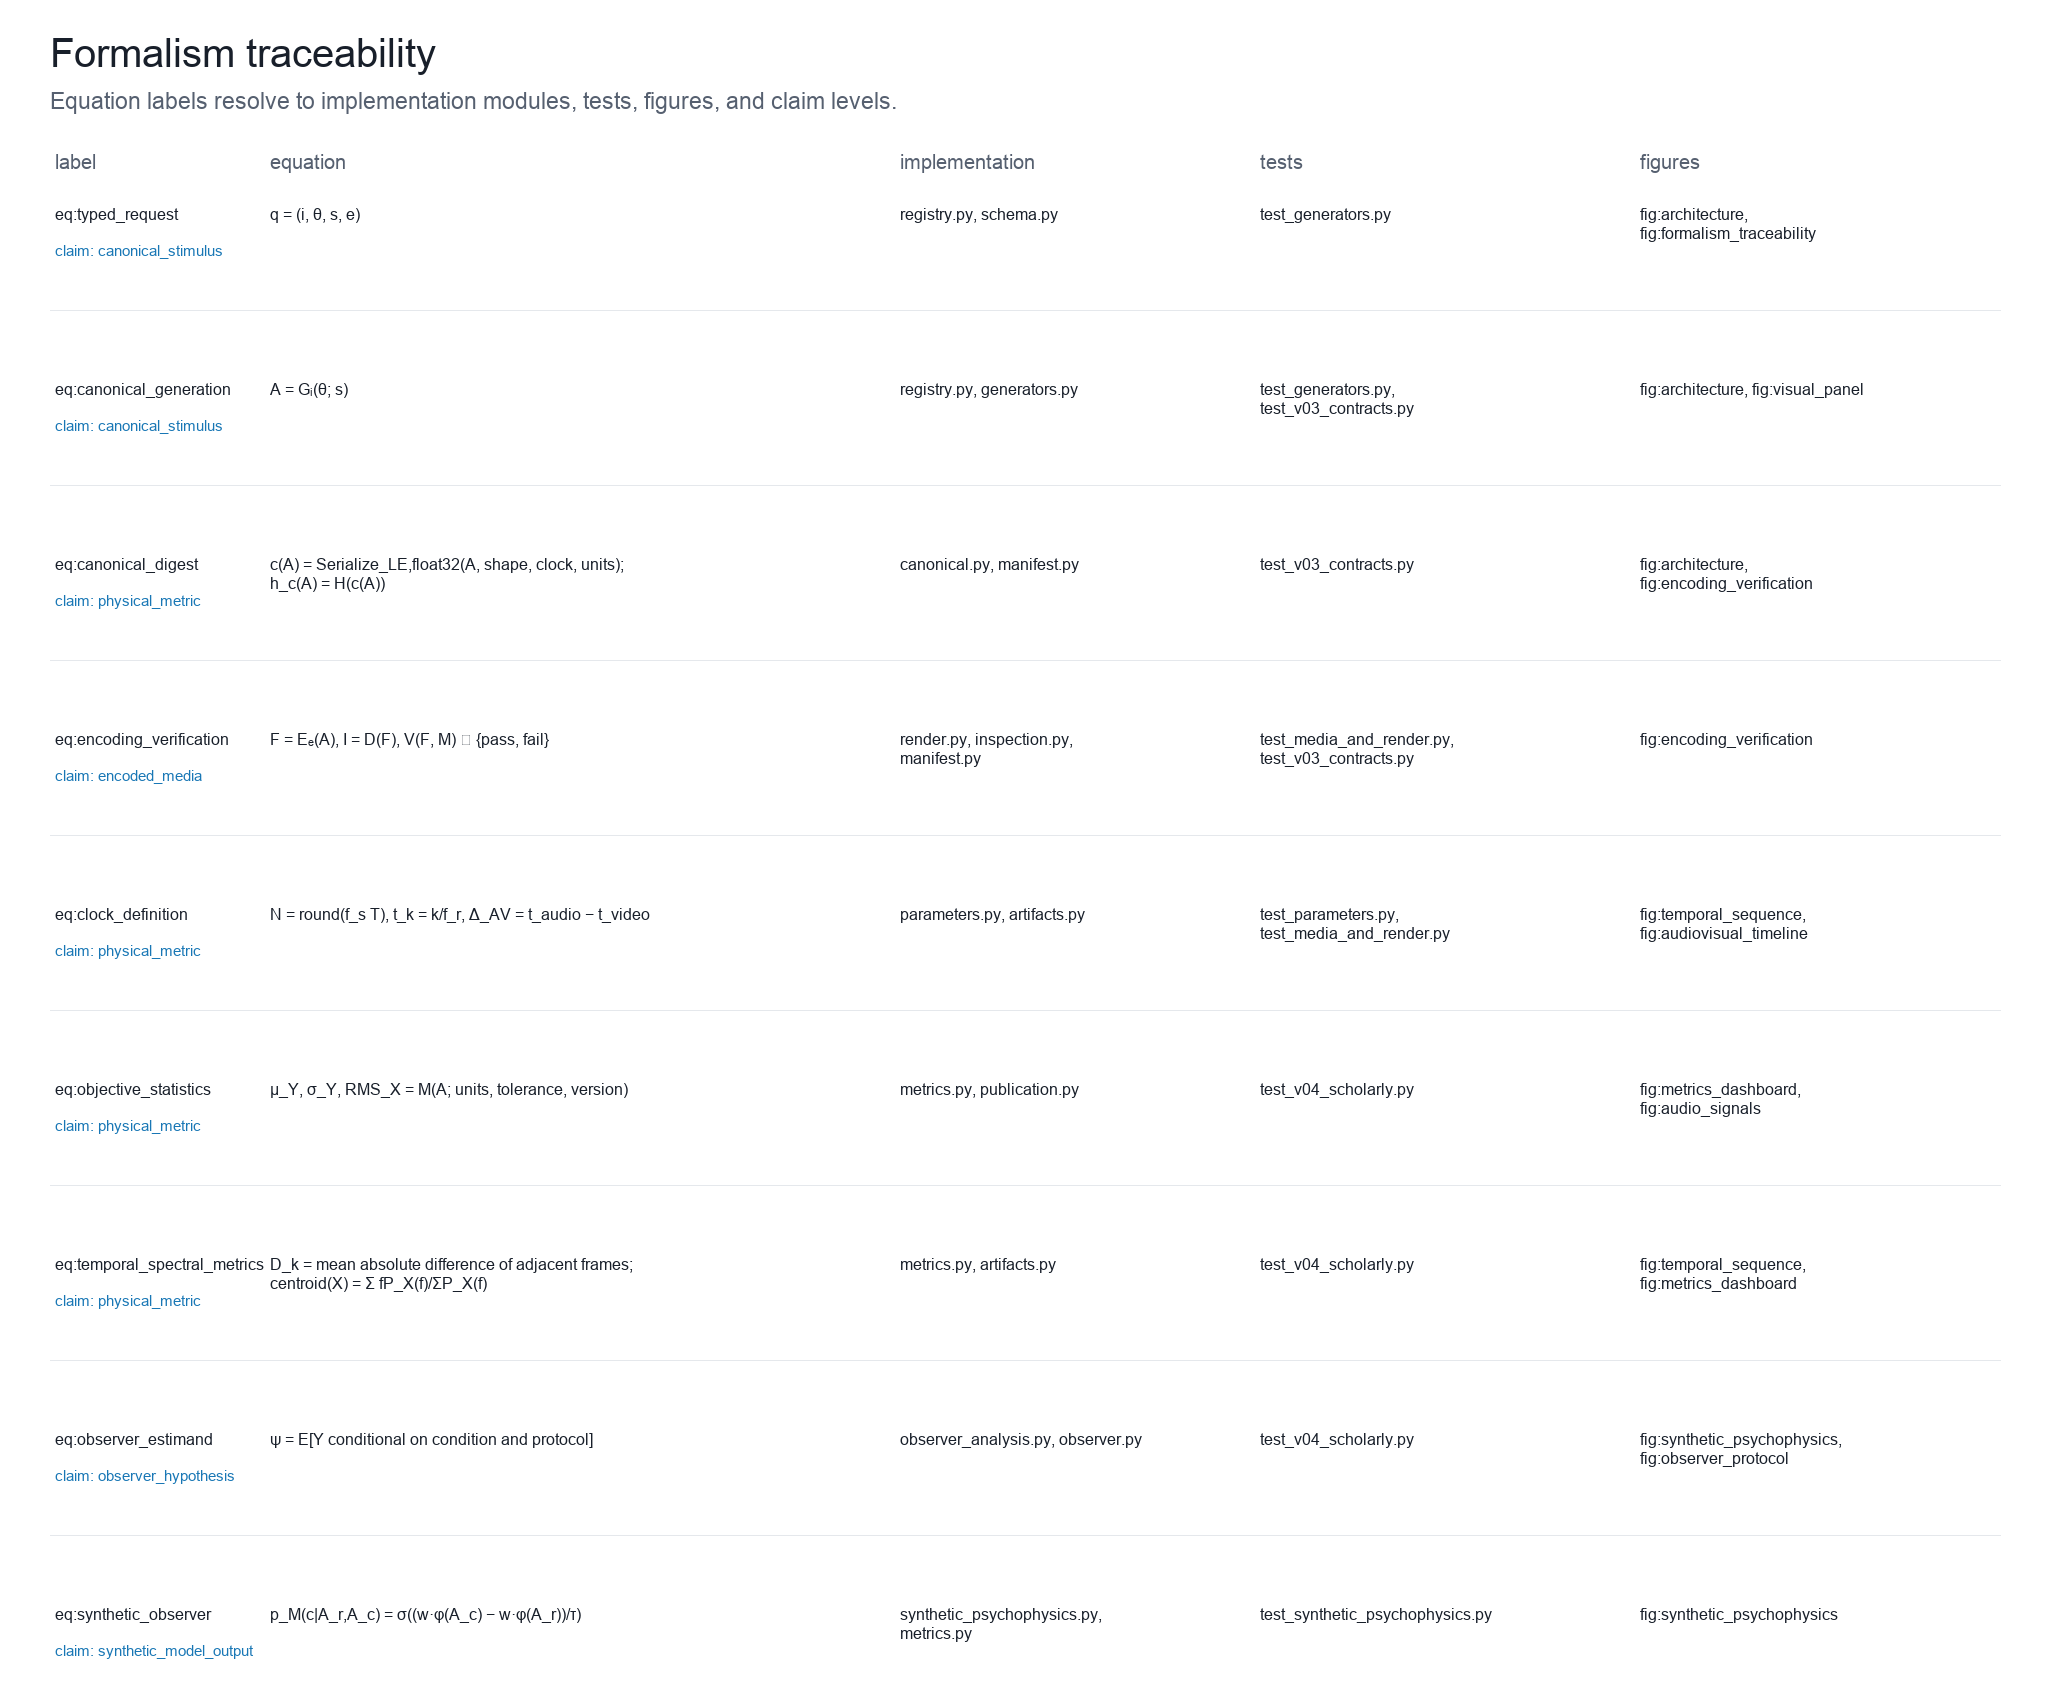
\includegraphics[keepaspectratio,alt={Rows connect equation labels to their mathematical definition, implementation paths, tests, figure labels, and claim levels.}]{../figures/formalism_traceability.png}}
\caption{Rows connect equation labels to their mathematical definition,
implementation paths, tests, figure labels, and claim
levels.}\label{fig:formalism_traceability}
\end{figure}

What this figure shows: Rows connect equation labels to their
mathematical definition, implementation paths, tests, figure labels, and
claim levels. The traceability registry connects the nine numbered
equations to symbols, implementation modules, tests, and registered
figures. Source data output/data/formalism\_traceability.json is the
machine-readable crosswalk used by the manuscript; it demonstrates
contract coverage and test linkage without converting formal notation
into empirical evidence. Controls: formalism registry version; seed not
applicable to the traceability diagram. Objective facts: nine equation
records with implementation, test, figure, and claim-level fields; no
unit-bearing measurement is plotted. Claim level: physical\_metric.
Source data: output/data/formalism\_traceability.json (SHA-256 digest
recorded in the figure registry). Evidence lineage:
formalism:eq:canonical\_digest, formalism:eq:clock\_definition,
formalism:eq:objective\_statistics. Limitations: Traceability records
documentation and verification scope; it does not establish the truth of
an observer-level theory. Boundary: A linked equation and test can show
an implemented contract, not a validated perceptual law.

The formalism registry \breakseq{[@fig:formalism\_traceability]} links
equations \breakseq{[@eq:typed\_request; @eq:canonical\_generation;
@eq:canonical\_digest; @eq:encoding\_verification;
@eq:clock\_definition; @eq:objective\_statistics;
@eq:temporal\_spectral\_metrics; @eq:observer\_estimand;
@eq:synthetic\_observer]} to implementation modules, tests, and
figures. The contract is intentionally auditable: equation labels point
to code-owned records, while empirical claims remain outside the
generator's authority.

\begin{figure}
\centering
\pandocbounded{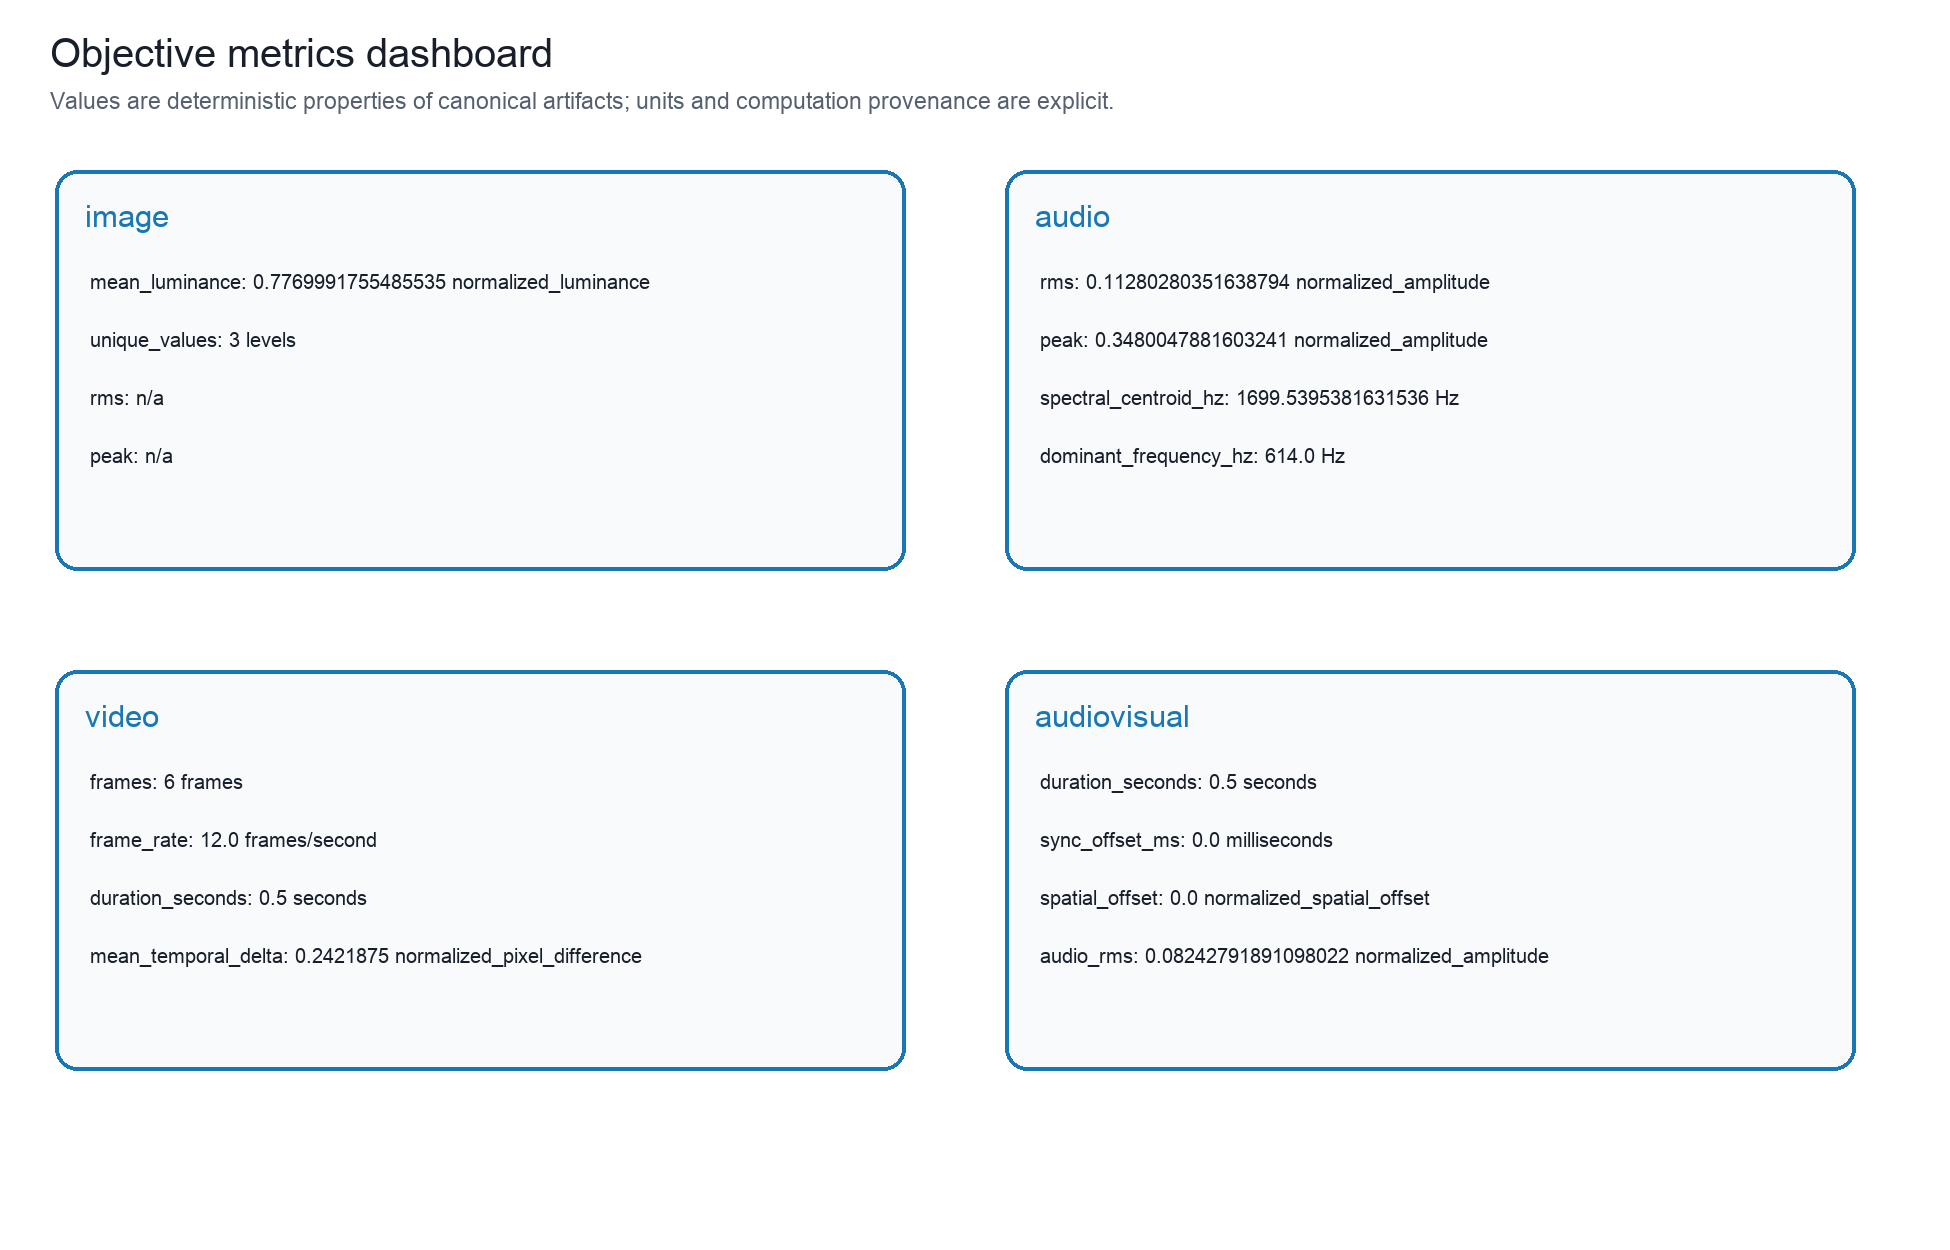
\includegraphics[keepaspectratio,alt={Four artifact cards list image, audio, video, and audiovisual metrics with units, computation provenance, and claim level.}]{../figures/metrics_dashboard.png}}
\caption{Four artifact cards list image, audio, video, and audiovisual
metrics with units, computation provenance, and claim
level.}\label{fig:metrics_dashboard}
\end{figure}

What this figure shows: Four artifact cards list image, audio, video,
and audiovisual metrics with units, computation provenance, and claim
level. The dashboard presents representative measurements from image,
audio, video, and audiovisual canonical artifacts. Source data
output/data/metrics\_dashboard.json retains metric name, value, unit,
computation version, tolerance, claim level, and canonical digest;
luminance is normalized, amplitude is normalized, spectra are in hertz,
frame differences are normalized pixel differences, and synchronization
is in milliseconds. Controls: default canonical artifacts; metric
computation version and tolerance recorded in the source-data sidecar;
seed s=0. Objective facts: finite objective values with units:
normalized luminance/amplitude, Hz, normalized pixel difference, ms,
counts, and durations. Claim level: physical\_metric. Source data:
output/data/metrics\_dashboard.json (SHA-256 digest recorded in the
figure registry). Evidence lineage: formalism:eq:objective\_statistics,
formalism:eq:temporal\_spectral\_metrics. Limitations: Metrics are media
properties and do not encode pitch, size, motion, localization, binding,
or other observer interpretations. Boundary: Metric reproducibility is a
package property; interpretation as perception requires a separate
observer design and data.

The metrics dashboard \breakseq{[@fig:metrics\_dashboard]} reports units,
computation version, and canonical digests. Luminance statistics are
normalized raster properties; RMS and peak are normalized-amplitude
properties; spectral values are in Hz; frame deltas are normalized pixel
differences; and synchronization offsets are in milliseconds. None is a
psychophysical score.

\begin{figure}
\centering
\pandocbounded{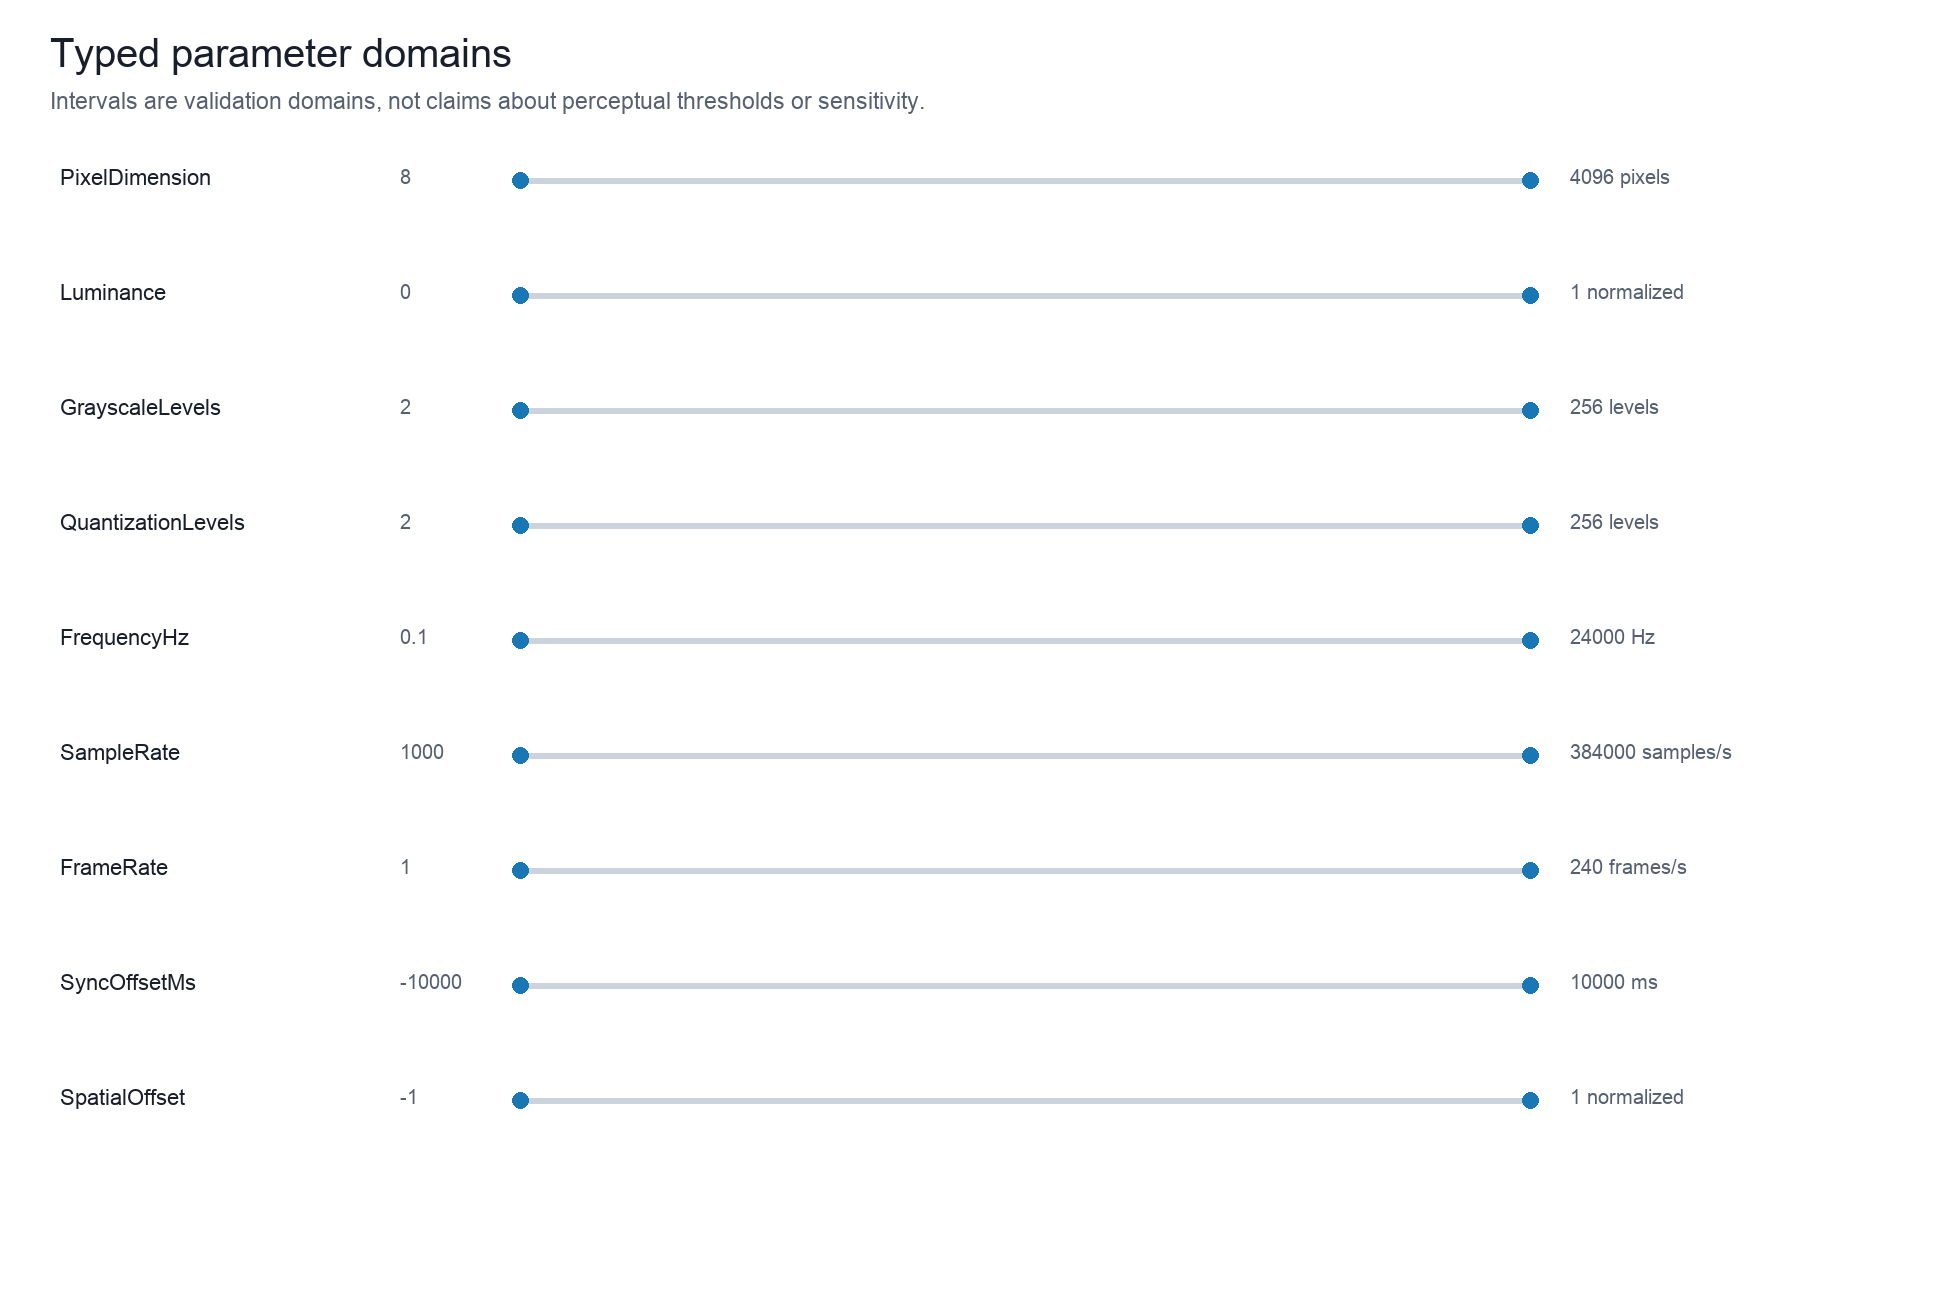
\includegraphics[keepaspectratio,alt={Horizontal interval markers show typed domains for dimensions, luminance, levels, frequency, sampling, frame rate, synchronization, and spatial discrepancy.}]{../figures/parameter_domains.png}}
\caption{Horizontal interval markers show typed domains for dimensions,
luminance, levels, frequency, sampling, frame rate, synchronization, and
spatial discrepancy.}\label{fig:parameter_domains}
\end{figure}

What this figure shows: Horizontal interval markers show typed domains
for dimensions, luminance, levels, frequency, sampling, frame rate,
synchronization, and spatial discrepancy. The domain map shows the
validated ranges for dimensions, luminance, grayscale and quantization
levels, frequency, sampling rate, frame rate, synchronization offset,
and spatial discrepancy. Source data output/data/parameter\_domains.json
records the type name, unit, interval, and engineering role; intervals
prevent malformed media and are not proposed as sensitivity thresholds.
Controls: parameter schema version and validated scalar domains; seed
not applicable to the domain diagram. Objective facts: dimensionless,
pixel, level, Hz, samples/s, frames/s, ms, and normalized spatial units
as listed per parameter. Claim level: canonical\_stimulus. Source data:
output/data/parameter\_domains.json (SHA-256 digest recorded in the
figure registry). Evidence lineage: formalism:eq:typed\_request.
Limitations: The intervals are software validation bounds and do not
encode safe listening levels, display limits, or psychophysical
thresholds. Boundary: A valid parameter is a reproducible construction
request, not evidence that the requested value is perceptually
effective.

The domain map \breakseq{[@fig:parameter\_domains]} is a validation
visualization. Bounds are chosen to prevent malformed media and unsafe
encodings, not to predict a viewer, listener, or participant's
sensitivity.
\end{frame}

\begin{frame}[fragile,allowframebreaks]{Observer-design boundary}
\protect\phantomsection\label{observer-design-boundary}
\begin{figure}
\centering
\pandocbounded{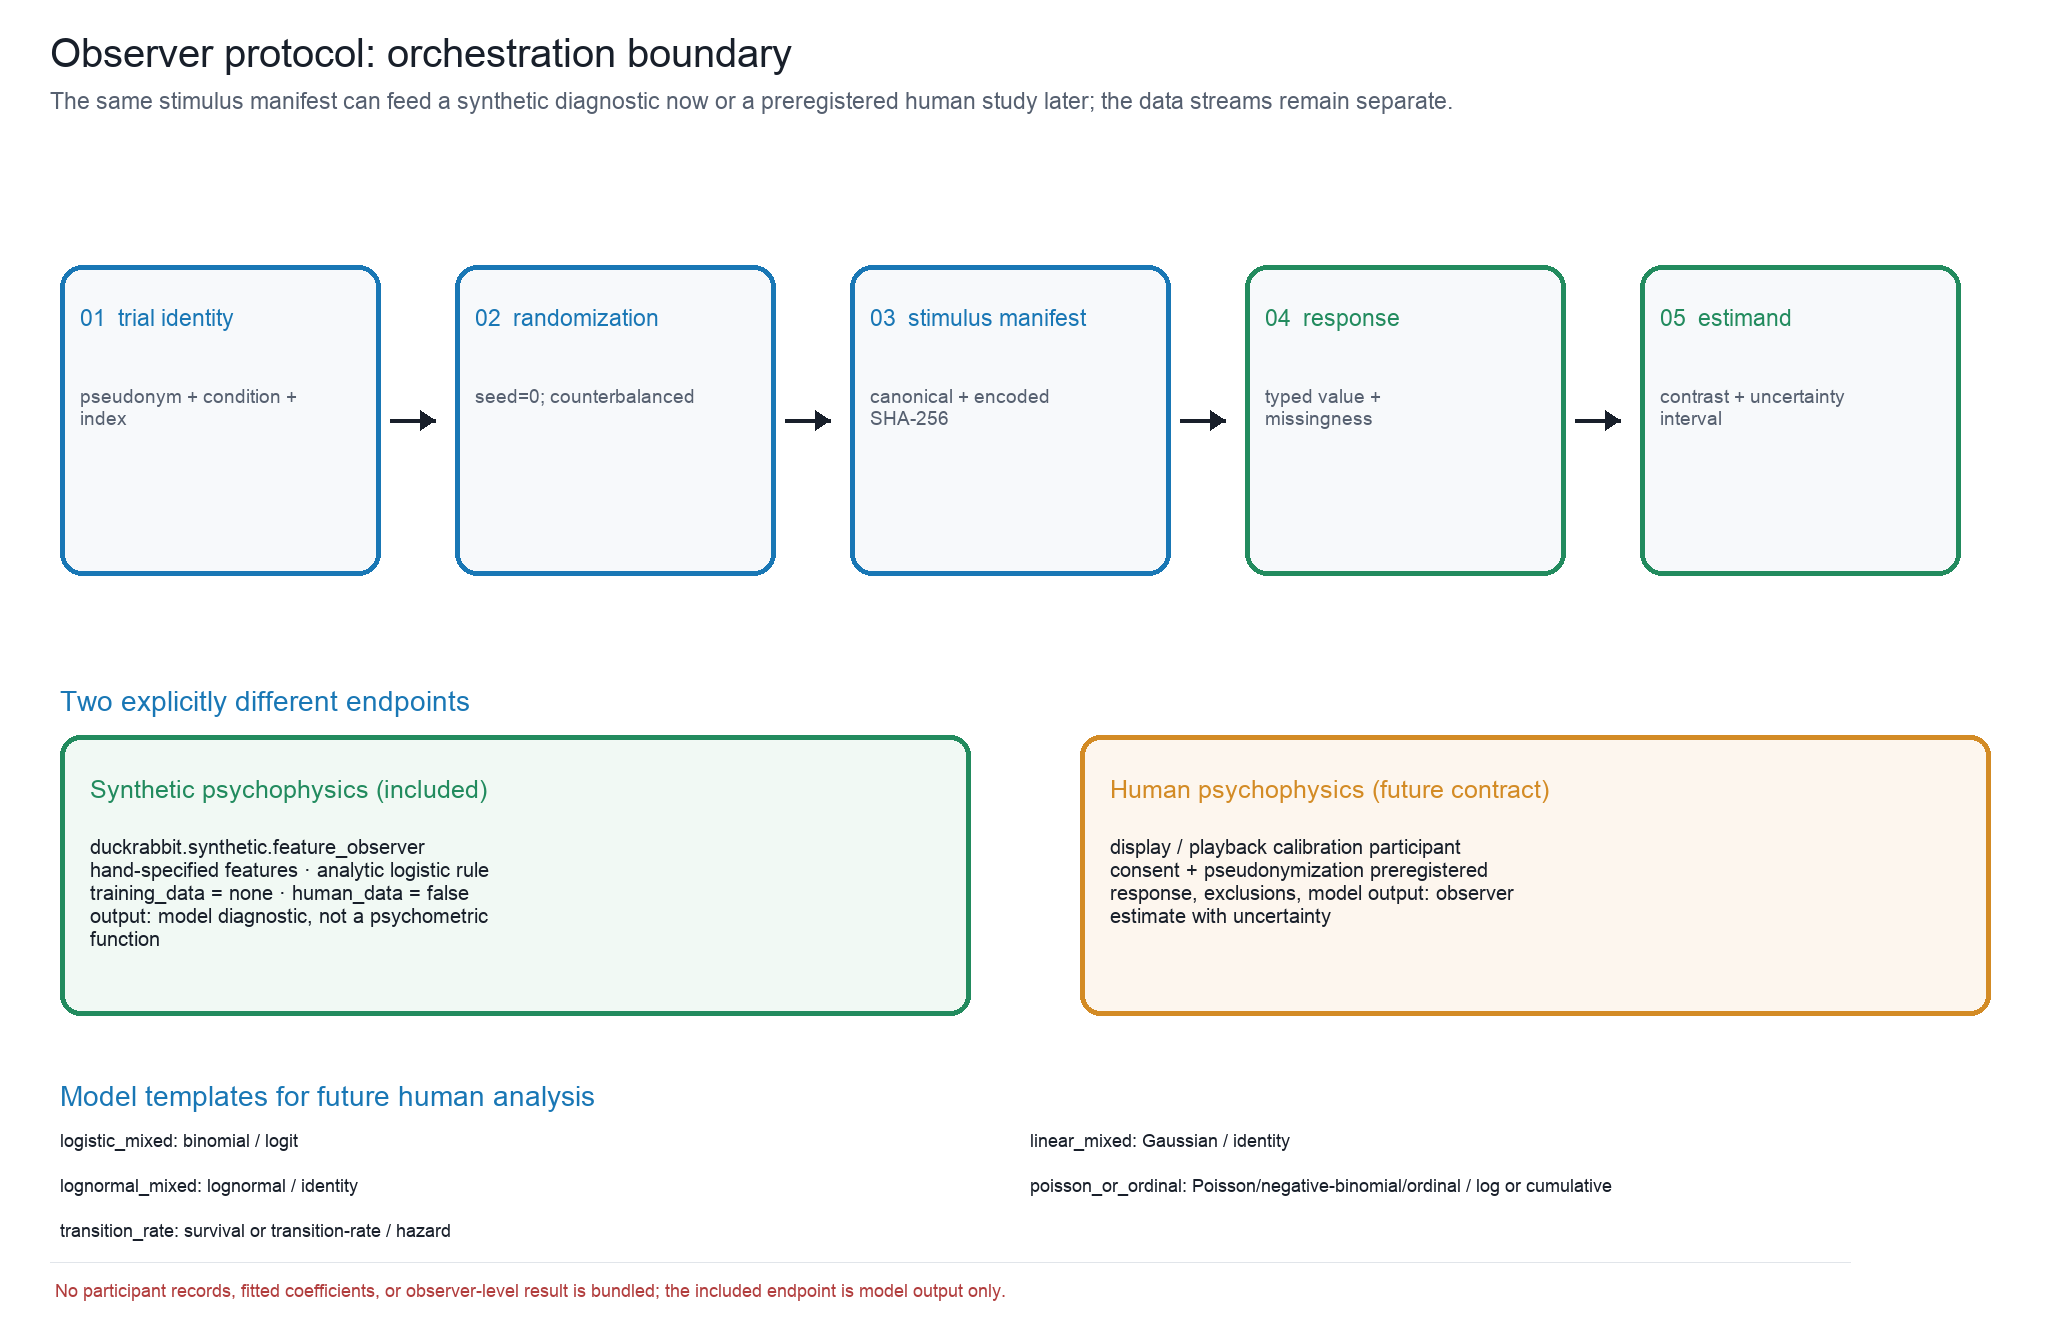
\includegraphics[keepaspectratio,alt={A flow diagram connects trial identity, randomization, stimulus manifest, response, aggregate estimand, and analysis-model templates, with a synthetic-only boundary.}]{../figures/observer_protocol.png}}
\caption{A flow diagram connects trial identity, randomization, stimulus
manifest, response, aggregate estimand, and analysis-model templates,
with a synthetic-only boundary.}\label{fig:observer_protocol}
\end{figure}

What this figure shows: A flow diagram connects trial identity,
randomization, stimulus manifest, response, aggregate estimand, and
analysis-model templates, with a synthetic-only boundary. The
study-ready scaffold moves from pseudonymous trial identity and
deterministic randomization to a stimulus manifest and encoded-file
hash, typed response or missingness, and a preregistered estimand.
Source data output/data/observer\_protocol.json records the study
design, randomization seed, model templates, and synthetic-only status;
no participant record is included. Controls: study design and
deterministic randomization seed recorded in the sidecar; synthetic
response generation is separate from human data. Objective facts: trial
counts, condition structure, estimand templates, response schemas, and
model families; participant outcomes are not applicable. Claim level:
observer\_hypothesis. Source data: output/data/observer\_protocol.json
(SHA-256 digest recorded in the figure registry). Evidence lineage:
observer:preregistered\_estimands. Limitations: The scaffold specifies
future data collection and analysis but supplies no participant
responses, fitted coefficients, power claim, or validated observer
effect. Boundary: The protocol is ready for ethical and preregistered
extension, not evidence that the proposed effect exists.

The observer scaffold \breakseq{[@fig:observer\_protocol]} starts with a
pseudonymous trial identity and deterministic randomization, binds the
stimulus manifest and encoded hash, records a typed response or
missingness state, and ends at a preregistered estimand. The companion
diagnostic \breakseq{[@fig:synthetic\_psychophysics]} is a deterministic,
hand-specified feature observer with \breaktt{training\_data=none} and
\breaktt{human\_data=false}; it is not a pretrained vision model,
psychometric function, or participant result. Human psychophysics
remains a future evidence layer requiring calibrated playback, consent,
preregistration, and observed responses.
\end{frame}

\begin{frame}[fragile,allowframebreaks]{Generated audit tables}
\protect\phantomsection\label{generated-audit-tables}
\begin{longtable}[]{@{}
  >{\raggedright\arraybackslash}p{(\linewidth - 6\tabcolsep) * \real{0.2500}}
  >{\raggedright\arraybackslash}p{(\linewidth - 6\tabcolsep) * \real{0.2500}}
  >{\raggedright\arraybackslash}p{(\linewidth - 6\tabcolsep) * \real{0.2500}}
  >{\raggedright\arraybackslash}p{(\linewidth - 6\tabcolsep) * \real{0.2500}}@{}}
\caption{Code-owned caption, source-data, and accessibility
audit.}\label{tbl:caption_audit}\tabularnewline
\toprule\noalign{}
\begin{minipage}[b]{\linewidth}\raggedright
Figure / claim level
\end{minipage} & \begin{minipage}[b]{\linewidth}\raggedright
Source and evidence
\end{minipage} & \begin{minipage}[b]{\linewidth}\raggedright
Controls and objective facts
\end{minipage} & \begin{minipage}[b]{\linewidth}\raggedright
Limitations, boundary, and accessibility
\end{minipage} \\
\midrule\noalign{}
\endfirsthead
\toprule\noalign{}
\begin{minipage}[b]{\linewidth}\raggedright
Figure / claim level
\end{minipage} & \begin{minipage}[b]{\linewidth}\raggedright
Source and evidence
\end{minipage} & \begin{minipage}[b]{\linewidth}\raggedright
Controls and objective facts
\end{minipage} & \begin{minipage}[b]{\linewidth}\raggedright
Limitations, boundary, and accessibility
\end{minipage} \\
\midrule\noalign{}
\endhead
fig:architecture; canonical stimulus & output/data/architecture.json;
formalism:eq:typed request, formalism:eq:canonical generation,
formalism:eq:encoding verification & Controls: typed request q=(i,θ,s,e)
with seed s=0; default generator and delivery-independent
canonicalization Objective: no unit-bearing objective quantity is
applicable to this architecture diagram; stage identities and provenance
fields are recorded in the sidecar & Limitations: The schematic
abstracts implementation boundaries and does not represent an observer
study or a causal theory of perception. Boundary: The pipeline verifies
reproducible media facts, not what a person experiences. Accessibility:
Stage names, mathematical symbols, and arrow direction are printed
directly; color is redundant. \\
fig:catalog matrix; source supported & output/data/catalog matrix.json;
gregory1997visual, hirst2020sound, bruns2019ventriloquist & Controls:
live taxonomy registry; evidence matrix snapshot; seed not applicable to
the catalog diagram Objective: 18 catalog rows; categorical facets and
statuses; no observer-level quantity is applicable & Limitations:
Taxonomy facets are engineering classifications and remain provisional
where the literature supports competing accounts. Boundary: Catalog
coverage is bounded to this registered package and does not enumerate
all known illusions. Accessibility: Every status and facet is written as
text; color only reinforces the printed status. \\
fig:visual panel; canonical stimulus & output/data/visual panel.json;
gregory1997visual, brugger1999duckrabbit, howe2005muller,
morgan1999poggendorff, fisher1967ponzo, yildiz2022ponzo,
kanizsa1976contours, mruczek2015ebbinghaus, earle1995zollner,
wertheimer1912motion, sekuler1996wertheimer & Controls: one default
typed parameter object per implemented visual entry; seed s=0;
dimensions, luminance bounds, grayscale, and quantization controls
remain in each generator schema; temporal entries display their first
frame but retain sequence metrics Objective: per tile: mean and
standard-deviation relative luminance, unique raster levels, and
canonical SHA-256 digest; temporal entries additionally retain frame
count, frame rate, and frame deltas; definitions and units are in the
source data JSON & Limitations: The gallery is complete for implemented
visual entries in this package, not a complete survey of visual
illusions; literature families, historical displays, and DuckRabbit
rasters are not pixel-identical by default. Viewing scale, display
calibration, viewing distance, and observer conditions can change the
relevance of a construction; the gallery does not measure an observer's
perceptual report. Boundary: The figure establishes coverage of the
package's implemented visual constructions and their deterministic
raster facts. It does not establish that any viewer will perceive the
named signature, nor that the set is exhaustive of the visual-illusion
literature. Accessibility: Each tile is labeled by stable illusion ID
and accompanied by printed luminance, level-count, and digest fields;
color only reinforces grouping and is not required to identify a
stimulus. \\
fig:visual sweep; physical metric & output/data/visual sweep.json;
brugger1999duckrabbit, gregory1997visual & Controls: duck weight ∈
\{0,.25,.5,.75,1\}; grayscale=quantization ∈ \{2,4,8,16,32\}; seed s=0
Objective: 25 canonical rasters; unique levels, normalized mean
luminance, and effective dynamic range per cell & Limitations: The grid
is a sensitivity of the construction parameters, not a psychophysical
sensitivity curve or a validated observer effect. Boundary: The chosen
grid is an engineering sampling of the parameter domain and does not
imply an optimal or perceptually uniform spacing. Accessibility: Row and
column labels state the parameter values; numerical metrics and units
are available in the sidecar. \\
fig:temporal sequence; physical metric & output/data/temporal
sequence.json; wertheimer1912motion, sekuler1996wertheimer & Controls:
visual.apparent motion default typed parameters; frame rate and frame
count from the canonical sequence; seed s=0 Objective: timestamps in
seconds, frame rate in frames/s, frame count, rational timebase, and
adjacent-frame normalized pixel difference & Limitations: Frame
succession and frame deltas are physical file properties; playback
timing, display persistence, and motion reports require a controlled
observer task. Boundary: The figure documents temporal structure rather
than the presence, direction, or strength of perceived motion.
Accessibility: Frame index, seconds, frames per second, and
normalized-difference labels remain interpretable without color. \\
fig:audio signals; physical metric & output/data/audio signals.json;
shepard1984scale, zatorre2005missing, deutsch1986tritone,
repp1997tritone, deutsch1974octave, warren1970continuity,
riecke2011continuity & Controls: default typed audio parameters;
per-generator channel layout and sample rate; seed s=0; one-sided FFT
display with 48 sampled bins Objective: RMS and peak in normalized
amplitude; spectral centroid and bandwidth in Hz; sample rate in
samples/s; channel layout and canonical SHA-256 digest & Limitations:
Playback level, transducer response, dichotic separation, masker design,
and listener judgments are external to the canonical buffer. Boundary:
The figure compares generated signal properties and literature-linked
families; it does not establish pitch, continuity, or stream
organization for a listener. Accessibility: Waveform, spectral,
amplitude, and frequency labels are printed; bar color is not the sole
encoding. \\
fig:audiovisual timeline; physical metric & output/data/audiovisual
timeline.json; shams2000sifi, hirst2020sound, vroomen2004temporal,
hartcherobrien2011temporal & Controls: audiovisual.sound induced flash
default shared timeline; declared sync offset ΔAV and spatial offset;
seed s=0 Objective: video luminance and audio envelope on normalized
shared time; ΔAV in ms; spatial discrepancy in normalized units; frame
and sample clocks in the sidecar & Limitations: Display refresh, audio
hardware, event latency, and observer temporal binding are not measured
by this figure. Boundary: A shared-clock construction is not evidence
that observers bind the events at the declared or any other perceptual
time. Accessibility: The two channels, time axis, signed offset
convention, and normalized spatial discrepancy are labeled in text. \\
fig:encoding verification; encoded media & output/data/encoding
verification.json; engineering:typed media adapters & Controls: typed
encoding profile selected per artifact; overwrite and backend capability
checks; seed inherited from the stimulus request Objective: format
availability and verification scope are environment observations; NPZ is
exact while other formats are decoded and tolerance-checked &
Limitations: Backend availability, codec versions, container metadata,
and lossy tolerances are environment-dependent; playback software can
expose additional behavior. Boundary: A successful encode or decode does
not validate an observer effect or guarantee cross-device perceptual
equivalence. Accessibility: Format, backend, preserved fact, and
verification columns are textual and remain usable without color. \\
fig:synthetic psychophysics; synthetic model output &
output/data/synthetic psychophysics.json; observer:preregistered
estimands & Controls: duck weight comparison against fixed reference;
serialized feature weights and temperature; seed s=0 Objective: model
probability and score delta on the displayed model-output scale;
canonical stimulus digests; human data=false; training data=none &
Limitations: The model is hand-specified, has no training data, has not
been calibrated against observers, and does not estimate a human
threshold or effect size. Its probabilities are model outputs, not
participant responses or a psychometric function. Boundary: This
diagnostic tests deterministic orchestration and metamorphic
input-output behavior only; empirical psychophysics remains future work.
Accessibility: Model scale, reference line, model identity, and
\breaktt{human\ data=false} are printed; color is not needed to interpret
the curve. \\
fig:claim boundary; source supported & output/data/claim boundary.json;
formalism:eq:observer estimand, formalism:eq:canonical digest &
Controls: claim levels in the taxonomy and manifest; seed not applicable
to the explanatory diagram Objective: no unit-bearing objective quantity
is applicable; stage definitions and evidence boundaries are preserved
in the sidecar & Limitations: The diagram is a documentation contract
and does not replace a preregistered observer study or empirical data.
Boundary: A deterministic artifact can support a future hypothesis but
cannot supply the observer data required to test it. Accessibility: Each
stage is named, numbered, and described in text; the boundary rule is
readable without color. \\
fig:scholarship map; source supported & output/data/scholarship
map.json; gregory1997visual, brugger1999duckrabbit, yildiz2022ponzo,
hirst2020sound, bruns2019ventriloquist & Controls: checked-in evidence
matrix; source roles and entry statuses; audit date recorded in
data/evidence matrix.json Objective: one evidence row per catalog entry
(18 entries); source-tier counts, exact claim text, engineering basis,
limitation, and gap status & Limitations: The offline snapshot validates
citation and lineage structure; live resolver status is a separate
audit, and classifications can remain contested. Boundary: Scholarship
coverage bounds the package's evidence record and does not establish
that any generated stimulus produces a universal percept. Accessibility:
Source roles, claims, limitations, and statuses are printed or available
in the sidecar; no category is encoded by color alone. \\
fig:formalism traceability; physical metric & output/data/formalism
traceability.json; formalism:eq:canonical digest, formalism:eq:clock
definition, formalism:eq:objective statistics & Controls: formalism
registry version; seed not applicable to the traceability diagram
Objective: nine equation records with implementation, test, figure, and
claim-level fields; no unit-bearing measurement is plotted &
Limitations: Traceability records documentation and verification scope;
it does not establish the truth of an observer-level theory. Boundary: A
linked equation and test can show an implemented contract, not a
validated perceptual law. Accessibility: Equation labels, code paths,
tests, and figure labels are written as text. \\
fig:metrics dashboard; physical metric & output/data/metrics
dashboard.json; formalism:eq:objective statistics, formalism:eq:temporal
spectral metrics & Controls: default canonical artifacts; metric
computation version and tolerance recorded in the source-data sidecar;
seed s=0 Objective: finite objective values with units: normalized
luminance/amplitude, Hz, normalized pixel difference, ms, counts, and
durations & Limitations: Metrics are media properties and do not encode
pitch, size, motion, localization, binding, or other observer
interpretations. Boundary: Metric reproducibility is a package property;
interpretation as perception requires a separate observer design and
data. Accessibility: Every numerical value is paired with a printed unit
or an explicit dimensionless definition. \\
fig:parameter domains; canonical stimulus & output/data/parameter
domains.json; formalism:eq:typed request & Controls: parameter schema
version and validated scalar domains; seed not applicable to the domain
diagram Objective: dimensionless, pixel, level, Hz, samples/s, frames/s,
ms, and normalized spatial units as listed per parameter & Limitations:
The intervals are software validation bounds and do not encode safe
listening levels, display limits, or psychophysical thresholds.
Boundary: A valid parameter is a reproducible construction request, not
evidence that the requested value is perceptually effective.
Accessibility: Type names, endpoints, units, and roles are printed;
interval color is redundant. \\
fig:observer protocol; observer hypothesis & output/data/observer
protocol.json; observer:preregistered estimands & Controls: study design
and deterministic randomization seed recorded in the sidecar; synthetic
response generation is separate from human data Objective: trial counts,
condition structure, estimand templates, response schemas, and model
families; participant outcomes are not applicable & Limitations: The
scaffold specifies future data collection and analysis but supplies no
participant responses, fitted coefficients, power claim, or validated
observer effect. Boundary: The protocol is ready for ethical and
preregistered extension, not evidence that the proposed effect exists.
Accessibility: Every protocol step and the no-participant-data boundary
is stated in text; arrows and labels remain legible without color. \\
\bottomrule\noalign{}
\end{longtable}

\begin{longtable}[]{@{}
  >{\raggedright\arraybackslash}p{(\linewidth - 8\tabcolsep) * \real{0.2000}}
  >{\raggedright\arraybackslash}p{(\linewidth - 8\tabcolsep) * \real{0.2000}}
  >{\raggedright\arraybackslash}p{(\linewidth - 8\tabcolsep) * \real{0.2000}}
  >{\raggedright\arraybackslash}p{(\linewidth - 8\tabcolsep) * \real{0.2000}}
  >{\raggedright\arraybackslash}p{(\linewidth - 8\tabcolsep) * \real{0.2000}}@{}}
\caption{Source-tiered evidence, DOI/URL verification, exact supported
claims, engineering departures, limitations, and explicit
planned/input-required gaps.}\label{tbl:evidence_audit}\tabularnewline
\toprule\noalign{}
\begin{minipage}[b]{\linewidth}\raggedright
Key
\end{minipage} & \begin{minipage}[b]{\linewidth}\raggedright
Record and citations
\end{minipage} & \begin{minipage}[b]{\linewidth}\raggedright
DOI and URL
\end{minipage} & \begin{minipage}[b]{\linewidth}\raggedright
Verification
\end{minipage} & \begin{minipage}[b]{\linewidth}\raggedright
Supported claim / engineering / limitation
\end{minipage} \\
\midrule\noalign{}
\endfirsthead
\toprule\noalign{}
\begin{minipage}[b]{\linewidth}\raggedright
Key
\end{minipage} & \begin{minipage}[b]{\linewidth}\raggedright
Record and citations
\end{minipage} & \begin{minipage}[b]{\linewidth}\raggedright
DOI and URL
\end{minipage} & \begin{minipage}[b]{\linewidth}\raggedright
Verification
\end{minipage} & \begin{minipage}[b]{\linewidth}\raggedright
Supported claim / engineering / limitation
\end{minipage} \\
\midrule\noalign{}
\endhead
gregory 1997 visual & review; gregory 1997 visual & DOI: recorded; URL
host/path: pubmed.ncbi.nlm.nih.gov & snapshot validated; offline
snapshot & A non-exhaustive classification of visual illusion
families. \\
hirst 2020 sound & review; hirst 2020 sound & DOI: recorded; URL
host/path: www.sciencedirect.com & snapshot validated; offline snapshot
& A review of sound-induced flash paradigms and multisensory temporal
inference. \\
howe 2005 muller & theory; howe 2005 muller & DOI: recorded; URL
host/path: doi.org & snapshot validated; offline snapshot & A
statistical image-source account of Müller-Lyer geometry. \\
morgan 1999 poggendorff & theory; morgan 1999 poggendorff & DOI:
recorded; URL host/path: doi.org & snapshot validated; offline snapshot
& A mechanistic account of Poggendorff orientation estimation. \\
fisher 1967 ponzo & primary; fisher 1967 ponzo & DOI: recorded; URL
host/path: www.nature.com & snapshot validated; offline snapshot & A
primary investigation of identical targets embedded in an angular
context. \\
kanizsa 1976 contours & primary; kanizsa 1976 contours & DOI: recorded;
URL host/path: pubmed.ncbi.nlm.nih.gov & snapshot validated; offline
snapshot & Canonical illusory-contour inducer arrangements. \\
mruczek 2015 ebbinghaus & primary; mruczek 2015 ebbinghaus & DOI:
recorded; URL host/path: pmc.ncbi.nlm.nih.gov & snapshot validated;
offline snapshot & Context-dependent size judgments in Ebbinghaus-family
stimuli. \\
wertheimer 1912 motion & primary; wertheimer 1912 motion & DOI: not
recorded; URL host/path: bibbase.org & snapshot validated; offline
snapshot & Foundational apparent-motion experiments using successive
spatial events. \\
sekuler 1996 wertheimer & review; sekuler 1996 wertheimer & DOI:
recorded; URL host/path: journals.sagepub.com & snapshot validated;
offline snapshot & A review connecting Wertheimer's successive-event
findings to later apparent-motion research and clarifying their
historical scope. \\
shepard 1984 scale & primary; shepard 1984 scale & DOI: recorded; URL
host/path: doi.org & snapshot validated; offline snapshot & Auditory
scale and pitch-class organization in Shepard-like tones. \\
zatorre 2005 missing & review; zatorre 2005 missing & DOI: recorded; URL
host/path: doi.org & snapshot validated; offline snapshot & The
missing-fundamental problem as a pitch-inference phenomenon. \\
deutsch 1986 tritone & primary; deutsch 1986 tritone & DOI: recorded;
URL host/path: online.ucpress.edu & snapshot validated; offline snapshot
& The tritone paradox and dependence on pitch-class context and
listener. \\
deutsch 1974 octave & primary; deutsch 1974 octave & DOI: recorded; URL
host/path: doi.org & snapshot validated; offline snapshot & Dichotic
alternating high/low tone construction underlying the octave
illusion. \\
shams 2000 sifi & primary; shams 2000 sifi & DOI: recorded; URL
host/path: doi.org & snapshot validated; offline snapshot & The
one-flash/two-beep sound-induced flash contrast. \\
bruns 2019 ventriloquist & review; bruns 2019 ventriloquist & DOI:
recorded; URL host/path: pmc.ncbi.nlm.nih.gov & snapshot validated;
offline snapshot & Spatial audiovisual capture and multisensory
integration constraints. \\
vroomen 2004 temporal & primary; vroomen 2004 temporal & DOI: recorded;
URL host/path: pubmed.ncbi.nlm.nih.gov & snapshot validated; offline
snapshot & Sound timing can alter the apparent temporal structure of a
visual event. \\
mcgurk 1976 speech & primary; mcgurk 1976 speech & DOI: recorded; URL
host/path: doi.org & snapshot validated; offline snapshot &
Speech-dependent audiovisual categorical integration, requiring
validated fixtures. \\
warren 1970 continuity & primary; warren 1970 continuity & DOI:
recorded; URL host/path: doi.org & snapshot validated; offline snapshot
& Auditory continuity/restoration as a future calibrated masker
family. \\
brugger 1999 duckrabbit & primary; brugger 1999 duckrabbit & DOI:
recorded; URL host/path: pubmed.ncbi.nlm.nih.gov & snapshot validated;
offline snapshot & Variation in duck/rabbit ambiguity across figure
variants and observers. \\
yildiz 2022 ponzo & review; yildiz 2022 ponzo & DOI: recorded; URL
host/path: pubmed.ncbi.nlm.nih.gov & snapshot validated; offline
snapshot & Competing depth-based and non-depth-based explanations of
Ponzo-like illusions. \\
repp 1997 tritone & primary; repp 1997 tritone & DOI: recorded; URL
host/path: pubmed.ncbi.nlm.nih.gov & snapshot validated; offline
snapshot & Listener- and context-dependent effects of spectral envelope
and pitch-class structure in tritone judgments. \\
hartcherobrien 2011 temporal & primary; hartcherobrien 2011 temporal &
DOI: recorded; URL host/path: pubmed.ncbi.nlm.nih.gov & snapshot
validated; offline snapshot & Audiovisual timing can shift temporal
judgments in a purely temporal context without spatial grounding. \\
earle 1995 zollner & primary; earle 1995 zollner & DOI: recorded; URL
host/path: journals.sagepub.com & snapshot validated; offline snapshot &
Crossing oblique and long-line geometry used to measure orientation
interactions in the Zöllner family. \\
zoellner 1860 pseudoscopy & primary; zoellner 1860 pseudoscopy & DOI:
recorded; URL host/path: onlinelibrary.wiley.com & snapshot validated;
offline snapshot & The nineteenth-century primary description of the
crossing-line orientation family later known as the Zöllner illusion. \\
riecke 2011 continuity & primary; riecke 2011 continuity & DOI:
recorded; URL host/path: doi.org & snapshot validated; offline snapshot
& Interrupted sounds with masking context and the separation of sensory
and decisional contributions. \\
wagemans 2012 gestalt & review; wagemans 2012 gestalt & DOI: recorded;
URL host/path: pubmed.ncbi.nlm.nih.gov & snapshot validated; offline
snapshot & Contemporary perceptual-grouping, contour-completion, and
figure-ground accounts relevant to Kanizsa-type constructions. \\
weintraub 1979 ebbinghaus & primary; weintraub 1979 ebbinghaus & DOI:
recorded; URL host/path: pubmed.ncbi.nlm.nih.gov & snapshot validated;
offline snapshot & A classic contextual-size experiment varying surround
geometry and comparison conditions in Ebbinghaus-family displays. \\
noppeney 2018 causal & review; noppeney 2018 causal & DOI: recorded; URL
host/path: doi.org & snapshot validated; offline snapshot &
Causal-inference and temporal-prediction accounts of audiovisual
integration and segregation. \\
alhazen 1989 optics & primary; alhazen 1989 optics & DOI: not recorded;
URL host/path: www.cca.qc.ca & snapshot validated; offline snapshot &
The English translation and commentary preserves Ibn al-Haytham's
eleventh-century Arabic optics as a historical source on direct vision
and geometrical image formation. \\
mozi 2023 canons & review; mozi 2023 canons & DOI: recorded; URL
host/path: link.springer.com & snapshot validated; offline snapshot & A
modern translation and commentary documents Mohist Canon sections on
knowledge, optics, and mechanics, providing a Chinese Warring
States-period context for early technical reasoning about vision. \\
ptolemy 1996 optics & primary; ptolemy 1996 optics & DOI: not recorded;
URL host/path: sites.dlib.nyu.edu & snapshot validated; offline snapshot
& The scholarly translation makes Ptolemy's second-century Optics
available as an early work on visual perception and mathematical visual
theory. \\
berkeley 1709 vision & primary; berkeley 1709 vision & DOI: not
recorded; URL host/path: www.maths.tcd.ie & snapshot validated; offline
snapshot & Berkeley's 1709 essay treats visual distance and space as
mediated by learned associations rather than as a simple direct readout
of visual geometry. \\
kircher 1646 light & primary; kircher 1646 light & DOI: not recorded;
URL host/path: collections.st-andrews.ac.uk & snapshot validated;
offline snapshot & The digitized record anchors Kircher's 1646 Ars magna
lucis et umbrae as an early-modern work on light, shadow, and optical
display. \\
molyneux 2020 problem & review; molyneux 2020 problem & DOI: not
recorded; URL host/path: plato.stanford.edu & snapshot validated;
offline snapshot & The historical account documents Molyneux's 1688
question separating tactile learning from visual recognition and its
long cross-sensory afterlife. \\
cheselden 1728 sight & primary; cheselden 1728 sight & DOI: not
recorded; URL host/path: archive.org & snapshot validated; offline
snapshot & The digitized Philosophical Transactions record preserves
Cheselden's 1728 case report as a historical observation relevant to
visual access and the separation of observer evidence from stimulus
description. \\
dai 2015 chinesescience & review; dai 2015 chinesescience & DOI:
recorded; URL host/path: link.springer.com & snapshot validated; offline
snapshot & A history of Chinese science and technology surveys ancient
Chinese physics and records optical phenomena as part of a non-European
history of visual science. \\
entry / visual.duck rabbit & engineering / limitation / gap; brugger
1999 duckrabbit; gregory 1997 visual & DOI: n/a; URL host/path:
data/evidence\_matrix.json & snapshot validated; offline snapshot & The
entry instantiates a controllable ambiguous-figure stimulus family.
Engineering basis: Parameterized ambiguous silhouette; not a
pixel-identical reproduction of a historical plate. Limitation: The
generator verifies geometry and luminance, not bistable reports. Missing
contract: none \\
entry / visual.simultaneous contrast & engineering / limitation / gap;
gregory 1997 visual & DOI: n/a; URL host/path:
data/evidence\_matrix.json & snapshot validated; offline snapshot & The
physical center patches are matched while surround luminance differs.
Engineering basis: Equal central patches on unequal luminance surrounds.
Limitation: Display calibration and observer adaptation are not modeled.
Missing contract: none \\
entry / visual.apparent motion & engineering / limitation / gap;
wertheimer 1912 motion; sekuler 1996 wertheimer & DOI: n/a; URL
host/path: data/evidence\_matrix.json & snapshot validated; offline
snapshot & The sequence contains controlled successive spatial events.
Engineering basis: Alternating rectangular masks at a fixed rational
frame rate. Limitation: The artifact establishes temporal succession,
not perceived motion. Missing contract: none \\
entry / audio.shepard tone & engineering / limitation / gap; shepard
1984 scale & DOI: n/a; URL host/path: data/evidence\_matrix.json &
snapshot validated; offline snapshot & The audio contains octave-related
partials with controlled sweep parameters. Engineering basis: Additive
octave-spaced partials with a deterministic envelope. Limitation:
Playback transducers and listener pitch judgments are external. Missing
contract: none \\
entry / audio.missing fundamental & engineering / limitation / gap;
zatorre 2005 missing & DOI: n/a; URL host/path:
data/evidence\_matrix.json & snapshot validated; offline snapshot & The
nominal fundamental component is absent from the canonical spectrum.
Engineering basis: Harmonic components are synthesized while the nominal
fundamental is omitted. Limitation: Pitch completion is an
observer-level inference. Missing contract: none \\
entry / audiovisual.sound induced flash & engineering / limitation /
gap; shams 2000 sifi; hirst 2020 sound & DOI: n/a; URL host/path:
data/evidence\_matrix.json & snapshot validated; offline snapshot & The
declared beep/flash event counts and offsets are physically encoded.
Engineering basis: One flash paired with one or two timed beeps on a
shared clock. Limitation: The stimulus does not establish a reported
flash count. Missing contract: none \\
entry / audiovisual.ventriloquist & engineering / limitation / gap;
bruns 2019 ventriloquist; noppeney 2018 causal & DOI: n/a; URL
host/path: data/evidence\_matrix.json & snapshot validated; offline
snapshot & The audio and visual channels carry a declared spatial
discrepancy. Engineering basis: Stereo panning and visual displacement
encode a spatial discrepancy. Limitation: Perceived localization depends
on room, headphones, display, and observer. Missing contract: none \\
entry / visual.muller lyer & engineering / limitation / gap; gregory
1997 visual; howe 2005 muller & DOI: n/a; URL host/path:
data/evidence\_matrix.json & snapshot validated; offline snapshot & The
two bar lengths are equal in the canonical raster while wing geometry
varies. Engineering basis: Equal bars with controlled arrow-wing
geometry. Limitation: The chosen normalized geometry is one engineering
variant. Missing contract: none \\
entry / visual.poggendorff & engineering / limitation / gap; gregory
1997 visual; morgan 1999 poggendorff & DOI: n/a; URL host/path:
data/evidence\_matrix.json & snapshot validated; offline snapshot & The
occluder and diagonal continuation are generated from explicit geometry.
Engineering basis: A diagonal continuation is separated by a rectangular
occluder. Limitation: Alignment judgments and orientation filters are
not measured. Missing contract: none \\
entry / visual.ponzo & engineering / limitation / gap; fisher 1967
ponzo; yildiz 2022 ponzo & DOI: n/a; URL host/path:
data/evidence\_matrix.json & snapshot validated; offline snapshot &
Target bars are physically equal and rails converge toward a vanishing
region. Engineering basis: Equal target bars are placed inside
converging rails. Limitation: Perspective interpretation is observer-
and display-dependent. Missing contract: none \\
entry / visual.kanizsa triangle & engineering / limitation / gap;
kanizsa 1976 contours; wagemans 2012 gestalt & DOI: n/a; URL host/path:
data/evidence\_matrix.json & snapshot validated; offline snapshot & The
image contains incomplete inducers with no explicitly drawn triangle
edge. Engineering basis: Three incomplete circular inducers are
rasterized around a triangular gap. Limitation: Illusory contour
completion is not directly measured. Missing contract: none \\
entry / visual.ebbinghaus & engineering / limitation / gap; mruczek 2015
ebbinghaus; weintraub 1979 ebbinghaus & DOI: n/a; URL host/path:
data/evidence\_matrix.json & snapshot validated; offline snapshot &
Central target geometry is held equal while contextual circle geometry
differs. Engineering basis: Equal central targets are surrounded by
different context-circle sizes. Limitation: Perceived size depends on
viewing scale and context. Missing contract: none \\
entry / visual.zollner & engineering / limitation / gap; zoellner 1860
pseudoscopy; earle 1995 zollner; gregory 1997 visual & DOI: n/a; URL
host/path: data/evidence\_matrix.json & snapshot validated; offline
snapshot & The entry instantiates a controlled crossing-line orientation
stimulus family. Engineering basis: Vertical long lines crossed by short
oblique inducers with explicit normalized spacing and angle. Limitation:
The raster verifies line geometry, not orientation judgments or a
pixel-identical historical reproduction. Missing contract: none \\
entry / audio.tritone paradox & engineering / limitation / gap; deutsch
1986 tritone; repp 1997 tritone & DOI: n/a; URL host/path:
data/evidence\_matrix.json & snapshot validated; offline snapshot & The
canonical pair has an explicit half-octave frequency relation.
Engineering basis: Two octave-complex tones are separated by a
half-octave interval. Limitation: Ascending/descending reports vary
across listeners and contexts. Missing contract: none \\
entry / audio.octave illusion & engineering / limitation / gap; deutsch
1974 octave & DOI: n/a; URL host/path: data/evidence\_matrix.json &
snapshot validated; offline snapshot & The two channels receive
alternating octave-related tones. Engineering basis: Alternating high
and low tones are assigned to opposite stereo channels. Limitation: The
auditory percept depends on dichotic presentation and listener. Missing
contract: none \\
entry / audio.auditory continuity & engineering / limitation / gap;
warren 1970 continuity; riecke 2011 continuity & DOI: n/a; URL
host/path: data/evidence\_matrix.json & snapshot validated; offline
snapshot & The canonical audio contains a reproducible interruption
interval and masker family. Engineering basis: An interrupted sinusoidal
carrier is replaced during a declared gap by a deterministic tone or
white-noise masker with typed amplitude. Limitation: The generator
reports the physical interruption and masker, not a listener's
continuity judgment or sensory-versus-decisional effect. Missing
contract: none \\
entry / audiovisual.temporal ventriloquism & engineering / limitation /
gap; vroomen 2004 temporal; hartcherobrien 2011 temporal; hirst 2020
sound; noppeney 2018 causal & DOI: n/a; URL host/path:
data/evidence\_matrix.json & snapshot validated; offline snapshot &
Audio and video event timing and declared offset are deterministic and
inspectable. Engineering basis: A visual flash and audio click share a
clock with explicit offset. Limitation: The generated single-event pair
is a simplified engineering stimulus. Missing contract: none \\
entry / audiovisual.mcgurk & engineering / limitation / gap; mcgurk 1976
speech & DOI: n/a; URL host/path: data/evidence\_matrix.json & snapshot
validated; offline snapshot & The catalog identifies a speech-dependent
audiovisual family without claiming implementation. Engineering basis:
Requires validated speech audio/video fixtures and licensing records.
Limitation: No fixture, consent record, or perceptual validation
contract is bundled. Missing contract: A licensed or consented
checksummed speech audio/video fixture, synchronization contract, and
preregistered perceptual validation protocol are required. \\
\bottomrule\noalign{}
\end{longtable}

\begin{longtable}[]{@{}
  >{\raggedright\arraybackslash}p{(\linewidth - 6\tabcolsep) * \real{0.2500}}
  >{\raggedright\arraybackslash}p{(\linewidth - 6\tabcolsep) * \real{0.2500}}
  >{\raggedright\arraybackslash}p{(\linewidth - 6\tabcolsep) * \real{0.2500}}
  >{\raggedright\arraybackslash}p{(\linewidth - 6\tabcolsep) * \real{0.2500}}@{}}
\caption{Formal equation-to-code
traceability.}\label{tbl:formalism}\tabularnewline
\toprule\noalign{}
\begin{minipage}[b]{\linewidth}\raggedright
Label
\end{minipage} & \begin{minipage}[b]{\linewidth}\raggedright
Definition and symbols
\end{minipage} & \begin{minipage}[b]{\linewidth}\raggedright
Implementation and tests
\end{minipage} & \begin{minipage}[b]{\linewidth}\raggedright
Figures and claim level
\end{minipage} \\
\midrule\noalign{}
\endfirsthead
\toprule\noalign{}
\begin{minipage}[b]{\linewidth}\raggedright
Label
\end{minipage} & \begin{minipage}[b]{\linewidth}\raggedright
Definition and symbols
\end{minipage} & \begin{minipage}[b]{\linewidth}\raggedright
Implementation and tests
\end{minipage} & \begin{minipage}[b]{\linewidth}\raggedright
Figures and claim level
\end{minipage} \\
\midrule\noalign{}
\endhead
eq:typed request & q = (i, θ, s, e) Symbols: i, θ, s, e & Code:
registry.py, schema.py; Tests: test generators.py & Figures:
fig:architecture, fig:formalism traceability; Level: canonical
stimulus \\
eq:canonical generation & A = Gᵢ(θ; s) Symbols: A, Gᵢ, θ, s & Code:
registry.py, generators.py; Tests: test generators.py, test v03
contracts.py & Figures: fig:architecture, fig:visual panel; Level:
canonical stimulus \\
eq:canonical digest & c(A) = Serialize\_LE,float32(A, shape, clock,
units); h\_c(A) = H(c(A)) Symbols: c(A), h\_c, H & Code: canonical.py,
manifest.py; Tests: test v03 contracts.py & Figures: fig:architecture,
fig:encoding verification; Level: physical metric \\
eq:encoding verification & F = Eₑ(A), I = D(F), V(F, M) ∈ \{pass, fail\}
Symbols: F, Eₑ, D, I, V, M & Code: render.py, inspection.py,
manifest.py; Tests: test media and render.py, test v03 contracts.py &
Figures: fig:encoding verification; Level: encoded media \\
eq:clock definition & N = round(f\_s T), t\_k = k/f\_r, Δ\_AV = t\_audio
− t\_video Symbols: N, f\_s, T, t\_k, f\_r, Δ\_AV & Code: parameters.py,
artifacts.py; Tests: test parameters.py, test media and render.py &
Figures: fig:temporal sequence, fig:audiovisual timeline; Level:
physical metric \\
eq:objective statistics & μ\_Y, σ\_Y, RMS\_X = M(A; units, tolerance,
version) Symbols: μ\_Y, σ\_Y, RMS\_X, M & Code: metrics.py,
publication.py; Tests: test v04 scholarly.py & Figures: fig:metrics
dashboard, fig:audio signals; Level: physical metric \\
eq:temporal spectral metrics & D\_k = mean absolute difference of
adjacent frames; centroid(X) = Σ fP\_X(f)/ΣP\_X(f) Symbols: D\_k, P\_X,
f & Code: metrics.py, artifacts.py; Tests: test v04 scholarly.py &
Figures: fig:temporal sequence, fig:metrics dashboard; Level: physical
metric \\
eq:observer estimand & ψ = E{[}Y conditional on condition and
protocol{]} Symbols: ψ, Y, condition, protocol & Code: observer
analysis.py, observer.py; Tests: test v04 scholarly.py & Figures:
fig:synthetic psychophysics, fig:observer protocol; Level: observer
hypothesis \\
eq:synthetic observer & p\_M(c given A\_r,A\_c) = σ((w·φ(A\_c) −
w·φ(A\_r))/τ) Symbols: p\_M, c, A\_r, A\_c, w, φ, τ & Code: synthetic
psychophysics.py, metrics.py; Tests: test synthetic psychophysics.py &
Figures: fig:synthetic psychophysics; Level: synthetic model output \\
\bottomrule\noalign{}
\end{longtable}

\begin{longtable}[]{@{}
  >{\raggedright\arraybackslash}p{(\linewidth - 6\tabcolsep) * \real{0.2500}}
  >{\raggedright\arraybackslash}p{(\linewidth - 6\tabcolsep) * \real{0.2500}}
  >{\raggedright\arraybackslash}p{(\linewidth - 6\tabcolsep) * \real{0.2500}}
  >{\raggedright\arraybackslash}p{(\linewidth - 6\tabcolsep) * \real{0.2500}}@{}}
\caption{Claim ledger separating code-derived facts, scholarship,
engineering departures, limitations, scope, and observer
hypotheses.}\label{tbl:claim_ledger}\tabularnewline
\toprule\noalign{}
\begin{minipage}[b]{\linewidth}\raggedright
Claim ID
\end{minipage} & \begin{minipage}[b]{\linewidth}\raggedright
Claim and level
\end{minipage} & \begin{minipage}[b]{\linewidth}\raggedright
Basis
\end{minipage} & \begin{minipage}[b]{\linewidth}\raggedright
Lineage and limitation
\end{minipage} \\
\midrule\noalign{}
\endfirsthead
\toprule\noalign{}
\begin{minipage}[b]{\linewidth}\raggedright
Claim ID
\end{minipage} & \begin{minipage}[b]{\linewidth}\raggedright
Claim and level
\end{minipage} & \begin{minipage}[b]{\linewidth}\raggedright
Basis
\end{minipage} & \begin{minipage}[b]{\linewidth}\raggedright
Lineage and limitation
\end{minipage} \\
\midrule\noalign{}
\endhead
catalog:count & The catalog contains 18 entries. Level:
canonical\_stimulus & derived\_from\_code & Lineage: taxonomy entries()
Limitation: Catalog membership is not a completeness claim about all
known illusions. Manuscript: manuscript/09 appendix catalog.md \\
evidence:source count & The checked-in evidence matrix contains 36
source records. Level: source\_supported & checked\_in\_scholarship &
Lineage: data/evidence matrix.json::sources Limitation: The offline
snapshot does not imply that every URL is currently reachable or that a
source supports more than its exact record. Manuscript: manuscript/06
scope and related work.md \\
scope:no participant data & No participant data are bundled with the
package. Level: observer\_hypothesis & derived\_from\_code & Lineage:
experiments/observer protocol.md; output/data/synthetic
psychophysics.json Limitation: Future observer studies require
preregistration, consent, calibrated presentation, and separate data
governance. Manuscript: manuscript/07 publication audit.md \\
synthetic:diagnostic boundary & The synthetic observer is a
deterministic model-output diagnostic, not human psychophysics. Level:
synthetic\_model\_output & synthetic\_model\_output & Lineage:
src/duckrabbit/synthetic psychophysics.py; output/data/synthetic
psychophysics.json Limitation: The hand-specified model has no training
data and has not been calibrated against observers. Manuscript:
manuscript/02 methodology.md \\
cover:editorial boundary & The cover is a publication illustration, not
an experimental stimulus or observer result. Level:
publication\_illustration & publication\_illustration & Lineage:
output/reports/cover visualization.json Limitation: The editorial asset
is not part of the deterministic scientific stimulus registry.
Manuscript: manuscript/07 publication audit.md \\
evidence:visual.duck rabbit & The entry instantiates a controllable
ambiguous-figure stimulus family. Level: source\_supported &
checked\_in\_scholarship & Lineage: sources=brugger1999duckrabbit;
gregory1997visual; data/evidence matrix.json; engineering=Parameterized
ambiguous silhouette; not a pixel-identical reproduction of a historical
plate.; limitation=The generator verifies geometry and luminance, not
bistable reports.; missing contract=none Limitation: The generator
verifies geometry and luminance, not bistable reports. Manuscript:
manuscript/06 scope and related work.md \\
evidence:visual.simultaneous contrast & The physical center patches are
matched while surround luminance differs. Level: source\_supported &
checked\_in\_scholarship & Lineage: sources=gregory1997visual;
data/evidence matrix.json; engineering=Equal central patches on unequal
luminance surrounds.; limitation=Display calibration and observer
adaptation are not modeled.; missing contract=none Limitation: Display
calibration and observer adaptation are not modeled. Manuscript:
manuscript/06 scope and related work.md \\
evidence:visual.apparent motion & The sequence contains controlled
successive spatial events. Level: source\_supported &
checked\_in\_scholarship & Lineage: sources=wertheimer1912motion;
sekuler1996wertheimer; data/evidence matrix.json;
engineering=Alternating rectangular masks at a fixed rational frame
rate.; limitation=The artifact establishes temporal succession, not
perceived motion.; missing contract=none Limitation: The artifact
establishes temporal succession, not perceived motion. Manuscript:
manuscript/06 scope and related work.md \\
evidence:audio.shepard tone & The audio contains octave-related partials
with controlled sweep parameters. Level: source\_supported &
checked\_in\_scholarship & Lineage: sources=shepard1984scale;
data/evidence matrix.json; engineering=Additive octave-spaced partials
with a deterministic envelope.; limitation=Playback transducers and
listener pitch judgments are external.; missing contract=none
Limitation: Playback transducers and listener pitch judgments are
external. Manuscript: manuscript/06 scope and related work.md \\
evidence:audio.missing fundamental & The nominal fundamental component
is absent from the canonical spectrum. Level: source\_supported &
checked\_in\_scholarship & Lineage: sources=zatorre2005missing;
data/evidence matrix.json; engineering=Harmonic components are
synthesized while the nominal fundamental is omitted.; limitation=Pitch
completion is an observer-level inference.; missing contract=none
Limitation: Pitch completion is an observer-level inference. Manuscript:
manuscript/06 scope and related work.md \\
evidence:audiovisual.sound induced flash & The declared beep/flash event
counts and offsets are physically encoded. Level: source\_supported &
checked\_in\_scholarship & Lineage: sources=shams2000sifi;
hirst2020sound; data/evidence matrix.json; engineering=One flash paired
with one or two timed beeps on a shared clock.; limitation=The stimulus
does not establish a reported flash count.; missing contract=none
Limitation: The stimulus does not establish a reported flash count.
Manuscript: manuscript/06 scope and related work.md \\
evidence:audiovisual.ventriloquist & The audio and visual channels carry
a declared spatial discrepancy. Level: source\_supported &
checked\_in\_scholarship & Lineage: sources=bruns2019ventriloquist;
noppeney2018causal; data/evidence matrix.json; engineering=Stereo
panning and visual displacement encode a spatial discrepancy.;
limitation=Perceived localization depends on room, headphones, display,
and observer.; missing contract=none Limitation: Perceived localization
depends on room, headphones, display, and observer. Manuscript:
manuscript/06 scope and related work.md \\
evidence:visual.muller lyer & The two bar lengths are equal in the
canonical raster while wing geometry varies. Level: source\_supported &
checked\_in\_scholarship & Lineage: sources=gregory1997visual;
howe2005muller; data/evidence matrix.json; engineering=Equal bars with
controlled arrow-wing geometry.; limitation=The chosen normalized
geometry is one engineering variant.; missing contract=none Limitation:
The chosen normalized geometry is one engineering variant. Manuscript:
manuscript/06 scope and related work.md \\
evidence:visual.poggendorff & The occluder and diagonal continuation are
generated from explicit geometry. Level: source\_supported &
checked\_in\_scholarship & Lineage: sources=gregory1997visual;
morgan1999poggendorff; data/evidence matrix.json; engineering=A diagonal
continuation is separated by a rectangular occluder.;
limitation=Alignment judgments and orientation filters are not
measured.; missing contract=none Limitation: Alignment judgments and
orientation filters are not measured. Manuscript: manuscript/06 scope
and related work.md \\
evidence:visual.ponzo & Target bars are physically equal and rails
converge toward a vanishing region. Level: source\_supported &
checked\_in\_scholarship & Lineage: sources=fisher1967ponzo;
yildiz2022ponzo; data/evidence matrix.json; engineering=Equal target
bars are placed inside converging rails.; limitation=Perspective
interpretation is observer- and display-dependent.; missing
contract=none Limitation: Perspective interpretation is observer- and
display-dependent. Manuscript: manuscript/06 scope and related
work.md \\
evidence:visual.kanizsa triangle & The image contains incomplete
inducers with no explicitly drawn triangle edge. Level:
source\_supported & checked\_in\_scholarship & Lineage:
sources=kanizsa1976contours; wagemans2012gestalt; data/evidence
matrix.json; engineering=Three incomplete circular inducers are
rasterized around a triangular gap.; limitation=Illusory contour
completion is not directly measured.; missing contract=none Limitation:
Illusory contour completion is not directly measured. Manuscript:
manuscript/06 scope and related work.md \\
evidence:visual.ebbinghaus & Central target geometry is held equal while
contextual circle geometry differs. Level: source\_supported &
checked\_in\_scholarship & Lineage: sources=mruczek2015ebbinghaus;
weintraub1979ebbinghaus; data/evidence matrix.json; engineering=Equal
central targets are surrounded by different context-circle sizes.;
limitation=Perceived size depends on viewing scale and context.; missing
contract=none Limitation: Perceived size depends on viewing scale and
context. Manuscript: manuscript/06 scope and related work.md \\
evidence:visual.zollner & The entry instantiates a controlled
crossing-line orientation stimulus family. Level: source\_supported &
checked\_in\_scholarship & Lineage: sources=zoellner1860pseudoscopy;
earle1995zollner; gregory1997visual; data/evidence matrix.json;
engineering=Vertical long lines crossed by short oblique inducers with
explicit normalized spacing and angle.; limitation=The raster verifies
line geometry, not orientation judgments or a pixel-identical historical
reproduction.; missing contract=none Limitation: The raster verifies
line geometry, not orientation judgments or a pixel-identical historical
reproduction. Manuscript: manuscript/06 scope and related work.md \\
evidence:audio.tritone paradox & The canonical pair has an explicit
half-octave frequency relation. Level: source\_supported &
checked\_in\_scholarship & Lineage: sources=deutsch1986tritone;
repp1997tritone; data/evidence matrix.json; engineering=Two
octave-complex tones are separated by a half-octave interval.;
limitation=Ascending/descending reports vary across listeners and
contexts.; missing contract=none Limitation: Ascending/descending
reports vary across listeners and contexts. Manuscript: manuscript/06
scope and related work.md \\
evidence:audio.octave illusion & The two channels receive alternating
octave-related tones. Level: source\_supported &
checked\_in\_scholarship & Lineage: sources=deutsch1974octave;
data/evidence matrix.json; engineering=Alternating high and low tones
are assigned to opposite stereo channels.; limitation=The auditory
percept depends on dichotic presentation and listener.; missing
contract=none Limitation: The auditory percept depends on dichotic
presentation and listener. Manuscript: manuscript/06 scope and related
work.md \\
evidence:audio.auditory continuity & The canonical audio contains a
reproducible interruption interval and masker family. Level:
source\_supported & checked\_in\_scholarship & Lineage:
sources=warren1970continuity; riecke2011continuity; data/evidence
matrix.json; engineering=An interrupted sinusoidal carrier is replaced
during a declared gap by a deterministic tone or white-noise masker with
typed amplitude.; limitation=The generator reports the physical
interruption and masker, not a listener's continuity judgment or
sensory-versus-decisional effect.; missing contract=none Limitation: The
generator reports the physical interruption and masker, not a listener's
continuity judgment or sensory-versus-decisional effect. Manuscript:
manuscript/06 scope and related work.md \\
evidence:audiovisual.temporal ventriloquism & Audio and video event
timing and declared offset are deterministic and inspectable. Level:
source\_supported & checked\_in\_scholarship & Lineage:
sources=vroomen2004temporal; hartcherobrien2011temporal; hirst2020sound;
noppeney2018causal; data/evidence matrix.json; engineering=A visual
flash and audio click share a clock with explicit offset.;
limitation=The generated single-event pair is a simplified engineering
stimulus.; missing contract=none Limitation: The generated single-event
pair is a simplified engineering stimulus. Manuscript: manuscript/06
scope and related work.md \\
evidence:audiovisual.mcgurk & The catalog identifies a speech-dependent
audiovisual family without claiming implementation. Level:
source\_supported & checked\_in\_scholarship & Lineage:
sources=mcgurk1976speech; data/evidence matrix.json;
engineering=Requires validated speech audio/video fixtures and licensing
records.; limitation=No fixture, consent record, or perceptual
validation contract is bundled.; missing contract=A licensed or
consented checksummed speech audio/video fixture, synchronization
contract, and preregistered perceptual validation protocol are required.
Limitation: No fixture, consent record, or perceptual validation
contract is bundled. Manuscript: manuscript/06 scope and related
work.md \\
publication:figure count & The publication atlas contains 15 registered
scientific figures. Level: physical\_metric & derived\_from\_code &
Lineage: publication caption specs() Limitation: The count is a
package-state fact, not evidence of empirical validity. Manuscript:
manuscript/07 publication audit.md \\
publication:table count & The publication appendix contains the
generated table set defined by the publication table payload registry.
Level: physical\_metric & derived\_from\_code & Lineage: publication
table payloads() Limitation: Generated tables summarize package state
and do not replace source or observer evidence. Manuscript:
manuscript/07 publication audit.md \\
\bottomrule\noalign{}
\end{longtable}

The source-tiered evidence table \breakseq{[@tbl:evidence\_audit]}, caption
audit \breakseq{[@tbl:caption\_audit]}, formalism registry
\breakseq{[@tbl:formalism]}, and claim ledger \breakseq{[@tbl:claim\_ledger]} are
generated sidecars. They provide a publication appendix without
duplicating mutable counts or silently converting literature statements
into package results.

The publication artifacts have two distinct provenance boundaries.
Scientific figures are deterministic PNG renders whose source-data JSON
and SHA-256 digests are checked against the code-owned registry. The
cover is an editorial charcoal illustration: its selected candidate,
prompt fingerprint, source asset digest, dimensions, variants, and
provenance boundary are recorded in
\breaktt{output/reports/cover\_visualization.json}. Neither boundary is
an observer result, and neither substitutes for display calibration or
behavioral data.

The publication audit additionally resolves every formalism edge to a
real package module, test file, manuscript equation label, and
registered figure. Figure source-data sidecars use a versioned schema
with figure identity, generator, seed, and nested data payload; the
registry verifies this identity and hash independently of the renderer.
This makes a visually plausible but stale or relabeled figure fail the
same provenance gate as a tampered stimulus.
\end{frame}

\end{document}
